%\documentclass[<options>]{elsarticle}
\documentclass [sort&compress] {elsarticle}
\usepackage{graphicx}% Include figure files

\bibliographystyle{elsarticle-num}
\begin{document}
\begin{frontmatter}

\title{Acoustically driven degradation in single crystalline silicon solar cell}

\author{O.Ya.~Olikh}
\ead{olikh@univ.kiev.ua}

\address{Faculty of Physics, Taras Shevchenko National University of Kyiv, Kyiv 01601, Ukraine}


\begin{abstract}
The influence of ultrasound on current--voltage characteristics of crystalline silicon solar sell was investigated experimentally.
The transverse and longitudinal acoustic waves were used over a temperature range of 290--340~K.
It was found that the ultrasound loading leads to the reversible decrease in the photogenerated current, open--circuit voltage, fill factor, carrier lifetime, and shunt resistance as well as the increase in the ideality factor.
The experimental results were described by using the models of coupled defect level recombination, Shockley--Read--Hall recombination, and dislocation--induced impedance.
The contribution of the boron-�oxygen related defects, iron-�boron pairs, and oxide precipitates to both the carrier recombination and acousto--defect interaction was discussed.
The experimentally observed phenomena are associated with the increase in the distance between coupled defects as well as the extension of the carrier capture coefficient of complex point defects and dislocations.
\end{abstract}

%\pacs{73.30.+y, 43.35.Ty, 43.35.+d, 72.20.-i, 73.40.-c}

\begin{keyword}
silicon\sep solar cells \sep ultrasound influence
\end{keyword}

\end{frontmatter}


\section{Introduction}

The silicon solar cells (SSCs) are still dominant in the photovoltaic field due to their high efficiency, low selling price and process maturity.
The material properties driving is a top priority for  most of manufacturers of SSC or another semiconductor  devices.
For example, the loss in the SSC efficiency is observed due to
illumination (the light--induced degradation or LID in the c--Si case \cite{LID:SchmidtJMR,LIDRev,LIDRev2,LID:JAP2017II} and the carrier-induced degradation or CID in the mc--Si case \cite{CID:APL,CID:PPS}),
high voltage (the potential--induced degradation or PID \cite{PID:SEMSC,PID:PP,PID:2017}),
or irradiation (the radiation--induced degradation or RID \cite{Bhat,Karazhanov}).
The degradation reason is a changing of crystal defects.
That is a transformation of the boron--oxygen or copper--contained complex (in LID case),
a decoration of the stacking faults by the positive ions, predominantly sodium, (in PID case) or
a creation of the radiation recombination centers (RID case).
The annealing at an elevated temperature is quite often required for efficiency recovery.

At the same time, the ultrasound (US) can effectively interact with defects in silicon.
It was experimentally observed that US can cause
transformation of impurity and radiation defects \cite{Korotchenkov1995,Ostapenko1995,Olikh2009Sem,UST:Medvid,Olikh2018JAP,YOlikh:SupMicr},
modification of  spectrum  \cite{Zaver:2008} and density \cite{Mirsagatov} of surface states,
changing of carrier diffusion length \cite{Ostapenko1999,Ostrovskii2001},
variation of current in  barrier structures \cite{OlikhJAP,Olikh2011Sem,Davletova2009,Davletova2008,YOlikh2005,Olikh:Ultras}.
Hence, it is expected that ultrasound--induced degradation (USID) can be originated by the acoustic wave (AW) action.
After AW propagation had stopped, the full recovery of material properties was often observed without annealing \cite{Ostapenko1999,Ostrovskii2001,OlikhJAP,Korotchenkov1995}.
Therefore, the USID is expected to be a reversible at room temperature in contrast to rest of degradations.



The aim of our work is to investigate experimentally the acoustically induced (AI) variation of  crystalline SSC photo--electrical parameters.
Ultrasound was found to result in a decrease in the solar cell efficiency.
The US intensity did not exceed $0.5$~W/cm$^2$ and the USID full recovery was observed at room temperature.
The USID dependencies on the AW both type and intensity are presented.
The experimentally observed phenomena are associated with the decrease in the carriers lifetime and in the shunt resistance as well as the increase in the ideality factor.
To describe the processes in the space charge region (SCR) and in the diode base as well as to study shunt resistance,
we used the models of coupled defect level recombination \cite{CDLR:JAP1995,CDLR:JAP},
Shockley--Read--Hall (SRH) recombination
and dislocation--induced impedance \cite{Rsh:Gopal2003,Rsh:Gopal2004}, respectively.
The observed AI phenomena are accounted for in terms of the defect interaction with the AW strain field \cite{MirzadeJAP2011,PeleshchakUJF2016}.




\section{Experimental and calculation details}
\subsection{Samples}

The SSC was fabricated from 2~in. (300~$\mu$m thick) p--type boron doped Czochralski silicon wafer with $<$111$>$ orientation and a doping level of $1.4\times10^{15}$~cm$^{-3}$.
The n$^+$ emitter with a carrier concentration of about $10^{19}$~cm$^{-3}$ and a thickness of 0.5~$\mu$m was formed by phosphorus implantation.
The wafer surface was capped by the TiO$_x$ antireflective coating.
The front and rear aluminium electrodes were deposited by screen printing before rapid annealing.
%The samples used in the experiment were cut from the central part of the wafer and had the area of $2$~cm$^{2}$.
%
%The investigated samples mainly differed in the shunt resistance ($R_{sh}$) value.
%The typical results for the samples with low ($R_{sh}\simeq10^4$~$\Omega\cdot$cm$^2$ at room temperature) and high ($R_{sh}>10^{15}$~$\Omega\cdot$cm$^2$) values are only presented in the article.
%These samples is labeled "SC4" and "SC15", respectively,  from now on.

The samples used in the experiment were cut from the wafer and mainly differed in the shunt resistance ($R_{sh}$) value.
The typical results for the samples with low ($R_{sh}\simeq10^4$~$\Omega\cdot$cm$^2$ at room temperature) and high ($R_{sh}>10^{15}$~$\Omega\cdot$cm$^2$) values are only presented in the article.
These samples is labeled ``SC4'' and ``SC15'', respectively,  from now on.


\subsection{Ultrasound loading}
In case of ultrasound loading (UL), the transverse or longitudinal AWs, which were exited by using LiNbO$_3$ piezoelectric transducer,  were applied to the samples at the base side in the [111]--direction.
The US frequencies $f_\mathtt{US}$, intensities $W_{\mathtt{US}}$, amplitudes of lattice deformation $\xi_{\mathtt{US}}=\sqrt{2W_\mathtt{US}/\rho_\mathtt{Si}\,\vartheta_{\mathtt{US}}^3}$, and lattice atom
displacements  $u_{\mathtt{US}}=\sqrt{W_\mathtt{US}/2\,\pi^2\,f_\mathtt{US}^2\,\rho_\mathtt{Si}\,\vartheta_{\mathtt{US}}}$ are listed in Table~\ref{tabUSL}.
$\rho_{Si}=2.33$~g/m$^3$ is the silicon density,
$\vartheta_{U\!S}$ is the US velocity, $9850$~m/s and $5840$~m/s in cases of longitudinal and transverse AWs, respectively.

\begin{table}
\caption{\label{tabUSL}The ultrasound loading parameters.
}
\begin{tabular}{ccccccc}
\hline
\hline
$f_\mathtt{US}$&wave&$W_{\mathtt{US}}$&$\xi_{\mathtt{US}}$&$u_{\mathtt{US}}$&UL&subjected\\
(MHz)&type&(W/cm$^2$)&($10^{-6}$)&(nm)&label&samples\\
\hline
8.0&longitudinal&0.18&1.3&0.3&lUL&SC4, SC15\\
4.2&transverse&0.19&2.8&0.6&tULa&SC15\\
4.2&transverse&0.22&3.1&0.7&tULb&SC4\\
4.2&transverse&0.40&4.2&0.9&tULc&SC4, SC15\\
\hline
\hline
\end{tabular}
\end{table}



It was reported previously \cite{Ostapenko1995,Olikh:Ultras,Ostrovskii2001} that the characteristic time of change in silicon structure parameters under
the US action  did not exceed $2\times10^3$~s.
In order to wait until the AI transitional period is competed, the following experimental procedure was used.
When UL started, the sample was first exposed to room temperature for 60~min and then the measurement and the sample heating were started.
In order to avoid the effect of piezoelectric field on both the measurements and sample parameters, the transducer was shielded.
The more details about the experimental setup are presented elsewhere \cite{Olikh:Ultras}.


\subsection{Current--voltage measurements and SSC parameters determination}

The dark and illuminated forward current--voltage ($J$--$V$) characteristics of the samples both with and without UL were measured over a temperature range of 290--340~K.
The temperature was controlled by differential copper--constantan thermocouple.
Some of the obtained curves are shown in Fig.~\ref{figIV}.

\begin{figure}
\begin{center}
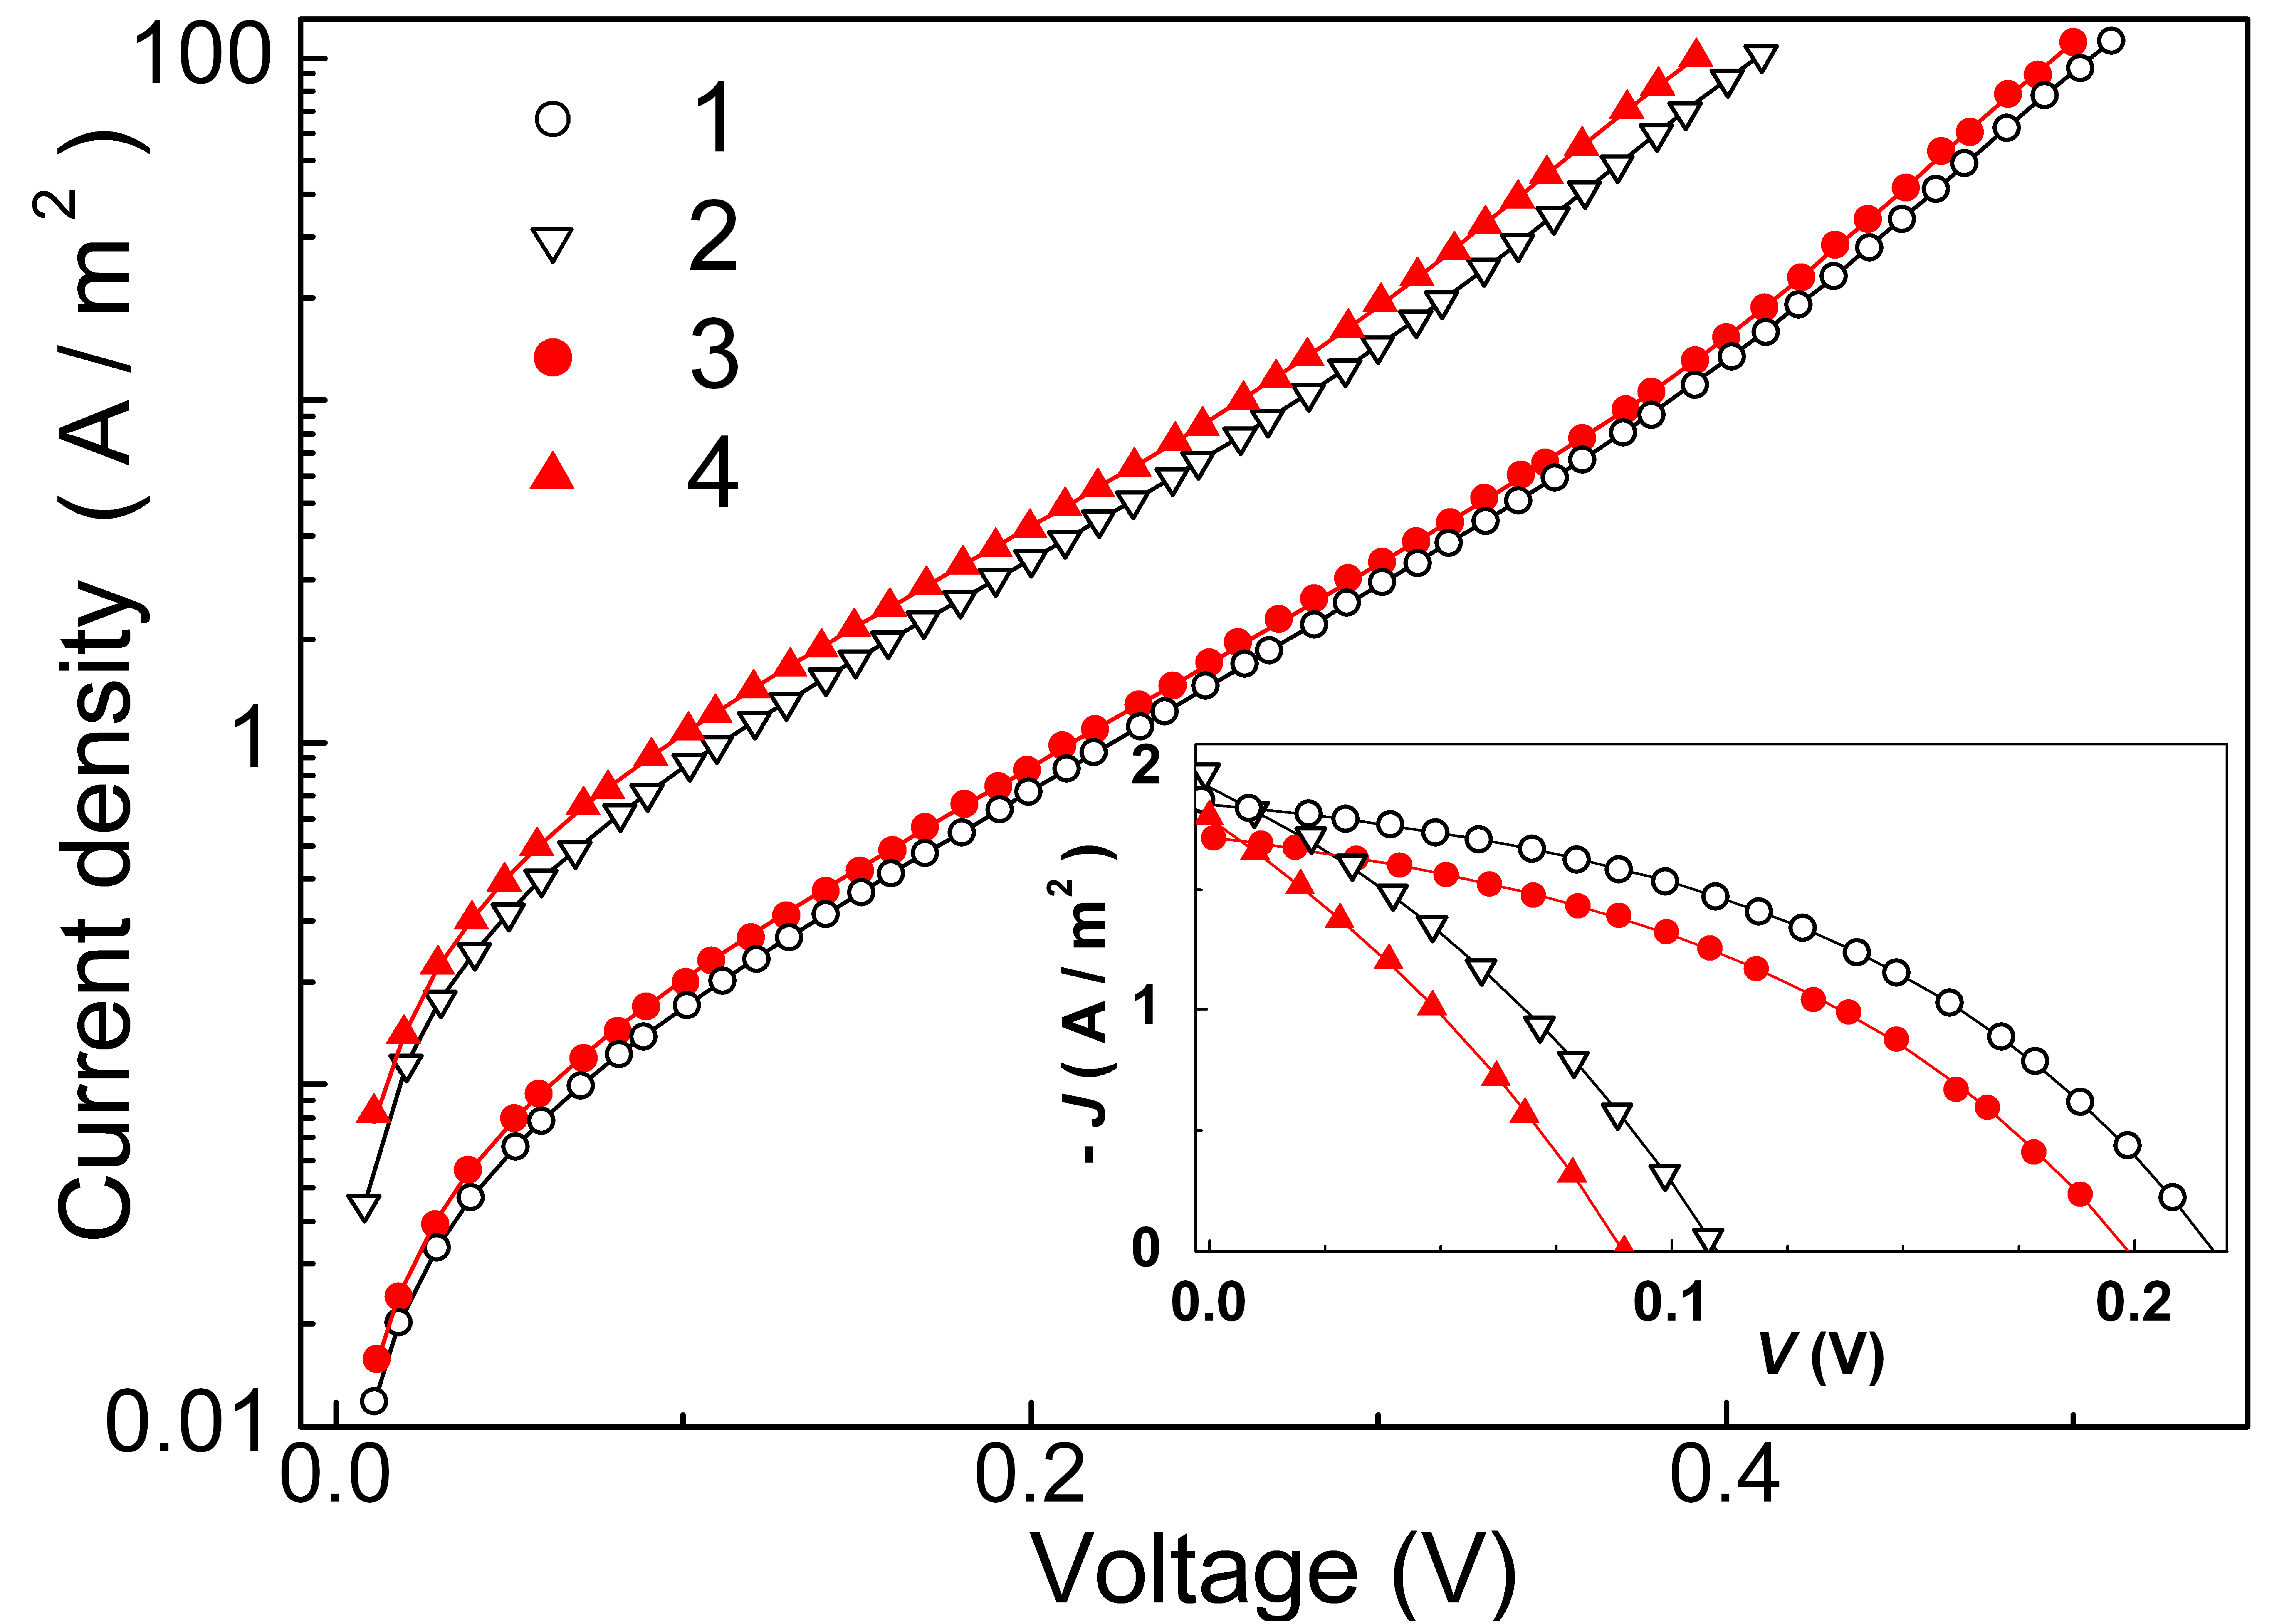
\includegraphics[width=9cm]{olikhFig1}%
\end{center}
\caption{\label{figIV}
Dark $J$--$V$ characteristics measured at 301~K (curves 1, 3, circles) and 341~K (curves 2, 4, triangles)
with (2, 4, filled marks, tULc) and without (1, 3, open marks) UL.
Inset: Parts of illuminated $J$--$V$ characteristics over a voltage range of 0--$V_{oc}$.
The marks are the experimental results, and the lines are the curves  fitted by Eqs.~(\ref{eqIV})--(\ref{eqW}).
}%
\end{figure}

The short--circuit current density $J_{sc}$, open--circuit voltage $V_{oc}$ and the fill factor $F\!F$ were estimated from the illuminated $J$--$V$ curve by the conventional mode.

The double--diode model of n$^+$--p SSC $J$--$V$ characteristics is expressed in the following form:
\begin{eqnarray}
\label{eqIV}
\nonumber J(V,T)&=&-J_{ph}+\frac{qn_id}{2\tau_{g}}\left\{\exp \left[\frac{q(V-JR_s)}{n_\mathrm{id}kT}\right]-1\right\}\\
&&+\frac{qn_i^2}{p_p}\sqrt{\frac{\mu_nkT}{\tau_n}}\left\{\exp \left[\frac{q(V-JR_s)}{kT}\right]-1\right\}+\frac{V-JR_s}{R_{sh}}\,,
\end{eqnarray}
where
$J_{ph}$ is the photogenerated current density,
$n_i$ is the intrinsic carrier concentration,
$\tau_{g}$ is the SCR carrier lifetime,
$d$ is the  SCR thickness:
\begin{equation}
\label{eqW}
    d(V,T)=\sqrt{\frac{2 \varepsilon \varepsilon_0(p_p+n_n)}{q p_p n_n}\left[\frac{E_g}{q}-\frac{kT}{q}\ln\left(\frac{N_vN_c}{p_pn_n}\right)-\frac{2kT}{q}-V\right]} \,,
\end{equation}
$\varepsilon$ is the permittivity (11.7 for Si),
$p_p$ and $n_n$ are the majority carrier concentration in the $p$-- and $n$--type regions,
$E_g$ is the semiconductor band gap,
$N_c$ and $N_v$ are the effective density of states in the conduction and valence bands;
$n_{\mathrm{id}}$ is the ideality factor,
$R_s$ is the series resistances,
and $\mu_n$ and $\tau_n$ are the mobility and lifetime of the electron (minority carrier) in the diode base.
The current-voltage  equation that models the solar cell by  an equivalent electrical circuit contains several parameters related to physical phenomena occurring in  the device.
It is commonly believed that $J_{0base}=(qn_i^2/n_n)\sqrt{\mu_nkT/\tau_n}$ is closely related to the recombination in the quasi--neutral region, while $J_{0SCR}=(qdn_i/2\tau_{g})$ describes the overall SCR recombination.


We used Eqs. (\ref{eqIV})--(\ref{eqW}) to fit the experimental data taking $\tau_g$, $\tau_n$, $n_{\mathrm{id}}$, $R_{sh}$, $R_s$, and  $J_{ph}$ (for illuminated $J$--$V$ curves only) as the  fitting parameters.
Also, we used the known \cite{ni:Green,Schroder2006,Markvart} temperature dependences of $n_i$, $E_g$, and $\mu_n$.
As a result, we obtained extremely good fit to the experimental data --- see Fig.~\ref{figIV}.
The parameters values, obtained from the dark and illuminated measurement at the same temperature and UL option, were identical practically.

It is known that $J_{sc}\approx J_{ph}R_{sh}/(R_{sh}+R_{s})$.
The value of $R_s$ was found to be about 2~$\Omega\cdot$cm$^2$, whereas $R_{sh}$ exceeded 4~k$\Omega\cdot$cm$^2$.
Therefore it is expected that $J_{sc}\approx J_{ph}$.
In fact, this relation was observed for the $J_{ph}$, which was obtained by fitting of whole of $J$--$V$ curve, and the $J_{sc}$, which was obtained as a point of intersection of a $J$--$V$ curve with a current axis.

To evaluate the US influence the relative change of parameters were used:
$\varepsilon_P=(P_{in}-P_\mathtt{US})/P_{in}$,
where $P$ is one of the set $\{J_{sc},V_{oc},F\!F,\tau_g,\tau_n,R_{sh}\}$,
subscripts ``$\mathtt{US}$'' and ``in'' indicate the values obtained at the same temperature with and without UL, respectively.
The AI change of the ideality factor was characterized by the absolute value $\Delta n_\mathrm{id}=n_{\mathrm{id},in}-n_{\mathrm{id},\mathtt{US}}$.


\subsection{Illumination}
The monochromatic ($\lambda=900$~nm) and low--intensity light was used for the SSCs illumination.
It is known \cite{BO:Halam2016} that illumination with intensity of above 0.01~suns can leads to defect formation in p--type silicon.
The our work was devoted to investigation of AI effects and the light intensity of $W_{ph}=(8\pm4)$~W/m$^2$ was chosen to avoid any current induced degradation processes.
The light monochromatism allowed to simplify the short--current dependence.
In case of used wavelength, the photocurrent defined  by the electron�-hole pairs generation in the $p$--region mainly.
If the base is several minority carrier diffusion lengths $L_n=\sqrt{\mu_nkT\tau_n/q}$, the $J_{sc}$ can be written as \cite{Markvart,Razeghi}
\begin{equation}
\label{eqIph}
J_{sc} = \frac{W_{ph}(1-M)q\beta\lambda}{hc}\frac{\alpha L_n}{1+ \alpha L_n}\,,
\end{equation}
where
$\alpha$ is the absorption coefficient,
$M$ is the reflection coefficient,
$\beta$ is the quantum yield coefficient.
We used Eq.~(\ref{eqIph}) to fit the experimental $J_{sc}(T)$ data taking $L_n$ as the fitting parameter.
Also, we used the known \cite{Markvart} temperature dependence of $\alpha$ and supposed that $\beta$ and $M$ were temperature independent, $L_n\propto T^{0.5}$.
The last relation was obtained from $J$--$V$ curves fitting --- see Sec.~\ref{P2}.
Thus, $L_n$ and $\tau_n$ can be obtained from the both single $J$--$V$ curve and $J_{sc}$ temperature dependence.
To to separate the second case values, the subscript ``$ph$'' was used: $L_n^{ph}$, $\tau_n^{ph}$, $\varepsilon_{\tau n}^{ph}$ etc.


\subsection{Fitting procedure}

All non-linear fittings were done by using the differential evolution method \cite{DE:Sun,DEWang,Olikh:Rev}.
The least--squares method was used to linear fitting.




\section{Results and Discussion}
\subsection{Photo--electric conversion}
The obtained temperature dependences of the the short--circuit current density, open--circuit voltage and the fill factor are shown in Fig.~\ref{figDUS_Isc}.
The parameters values at 320~K are listed in Tab.~\ref{tabParam}.
It should be noted that not only $I_{sc}$ and $V_{oc}$ but also SSC efficiency, $F\!F$, and minority carrier lifetime
decreases under low--intensity light conditions \cite{LI:Ruhle,LI:Reich,LI:lifetime}.
Hence, data in Fig.~\ref{figDUS_Isc} and Table~\ref{tabParam} are not equivalent to the standard test condition (AM1.5, $25^{\circ}$C, 1000~W/m$^2$) results,
but illustrate the AI effects.





\begin{figure}
\begin{center}
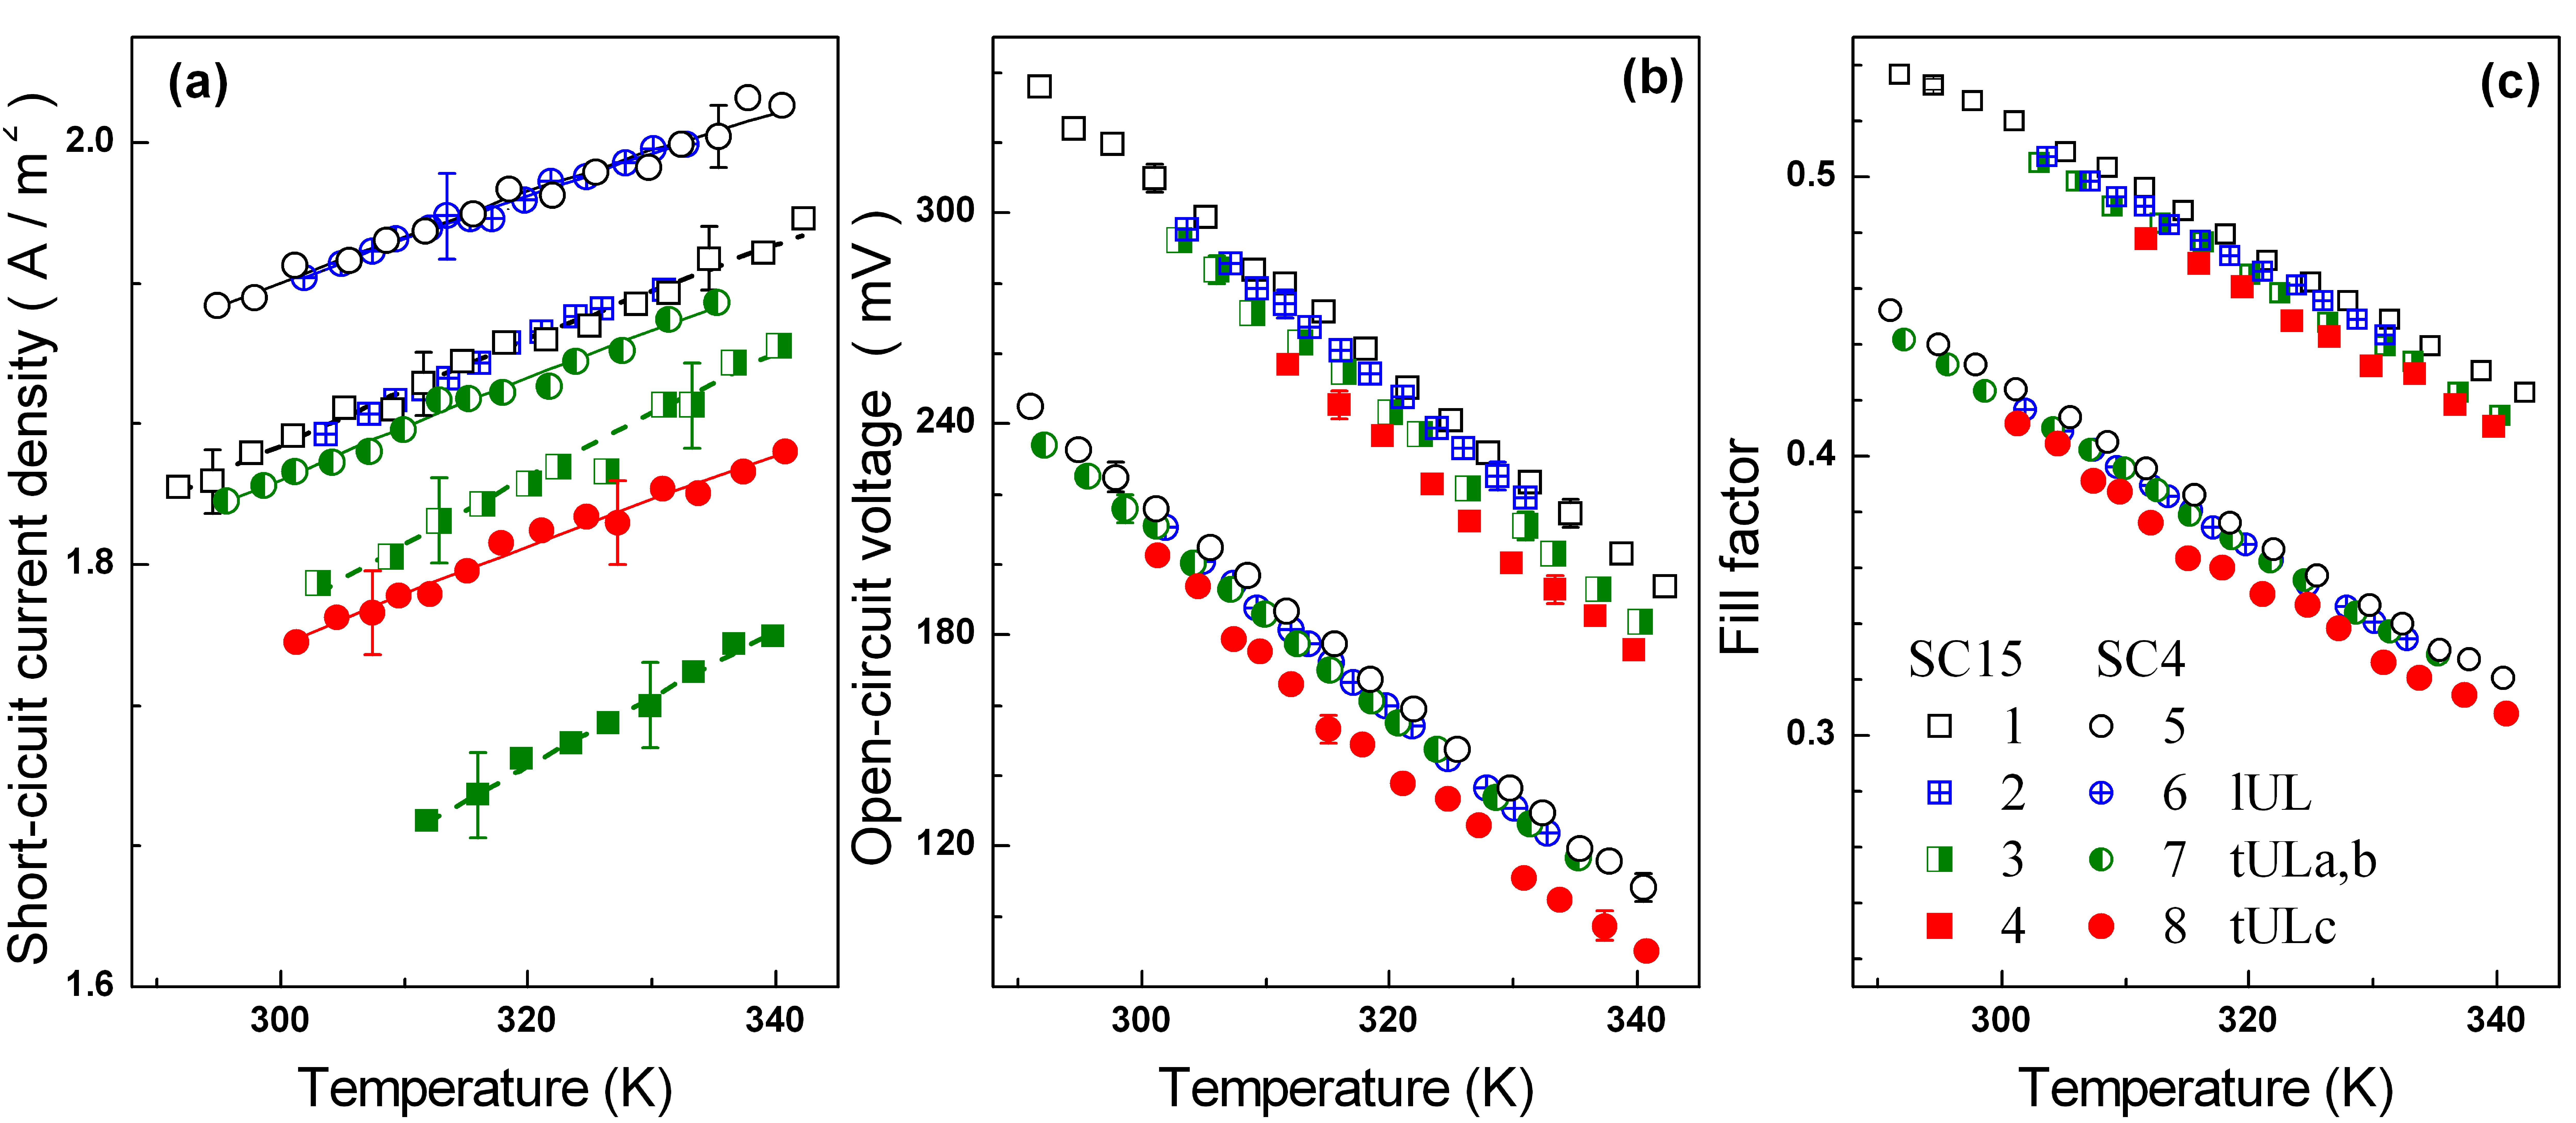
\includegraphics[width=14cm]{olikhFig2}%
\end{center}
\caption{\label{figDUS_Isc}
Temperature dependences of short--circuit (a),  open--circuit voltage (b) and  fill factor (c) for SC15 (squares) and SC4 (circles).
The curves 1 and 5 (open marks) are obtained without UL,
curves 2 and 6 correspond to lUL,
curve 3 corresponds to tULa,
curve 7 corresponds to tULb,
curves 4 and 8 correspond to tULc.
The marks are the experimental results, and the lines are the curves  fitted by Eq.~(\ref{eqIph}).
}%
\end{figure}


\begin{table}
\caption{\label{tabParam}The determined SSC parameters (at 320~K).
}
\begin{tabular}{lcccccccc}
\hline
\hline
&\multicolumn{4}{c}{SC15}&\multicolumn{4}{c}{SC4}\\
Parameter&\multicolumn{4}{c}{Ultrasound loading}&\multicolumn{4}{c}{Ultrasound loading}\\
&non&lUL&tULa&tULc&non&lUL&tULb&tULc\\
\hline
$J_{sc}$ (0.01A/m$^2$)&191$\pm$2&191$\pm$2&184$\pm$2&171$\pm$2&198$\pm$2&198$\pm$2&189$\pm$2&181$\pm$2\\
$V_{oc}$ (mV)&256$\pm$4&250$\pm$4&243$\pm$4&233$\pm$4&164$\pm$4&159$\pm$4&157$\pm$4&141$\pm$4\\
$F\!F$ ($10^{-3}$)&475$\pm$2&468$\pm$2&463$\pm$2&458$\pm$2&372$\pm$2&366$\pm$2&366$\pm$2&353$\pm$2\\
$L_n^{ph}$ ($\mu$m)$^*$&99$\pm$5&92$\pm$5&67$\pm$4&55$\pm$3&125$\pm$6&124$\pm$6&103$\pm$5&98$\pm$5\\
$L_n$ ($\mu$m)&93$\pm$5&82$\pm$4&47$\pm$3&34$\pm$2&106$\pm$5&99$\pm$5&80$\pm$4&69$\pm$4\\
$\tau_n^{ph}$ ($10^{-7}$ s)$^*$&31$\pm$3&26$\pm$3&14$\pm$2&9$\pm$1&49$\pm$5&48$\pm$5&33$\pm$4&30$\pm$3\\
$\tau_n$ ($10^{-7}$ s)&26$\pm$3&21$\pm$3&7$\pm$2&3.5$\pm$0.7&35$\pm$3&31$\pm$3&20$\pm$3&15$\pm$2\\
$\tau_g$ ($10^{-9}$ s)&70$\pm$4&66$\pm$3&57$\pm$3&48$\pm$2&35$\pm$2&31$\pm$2&30$\pm$2&29$\pm$2\\
$E_{\tau g}$ (meV)$^*$&242$\pm$7&237$\pm$5&234$\pm$5&234$\pm$5&246$\pm$6&234$\pm$5&241$\pm$5&243$\pm$5\\
$n_\mathrm{id}$ ($\pm$0.01)&2.59&2.60&2.61&2.63&2.51&2.52&2.54&2.54\\
$T_\mathrm{id}$ (K)$^*$&226$\pm$8&215$\pm$10&243$\pm$15&233$\pm$15&327$\pm$10&319$\pm$15&308$\pm$20&358$\pm$25\\
$K_\mathtt{US}$ (m$^{-2}$s$^{-1}$)&\multicolumn{4}{c}{(3.3$\pm$0.5)$\times10^{24}$}&\multicolumn{4}{c}{(5.0$\pm$0.2)$\times10^{23}$}\\
$R_{sh}$ (k$\Omega\cdot$cm$^2$)&$>10^{12}$&$>10^{12}$&$>10^{12}$&$>10^{12}$&12$\pm$1&13$\pm$1&10$\pm$1&8$\pm$1\\
\hline
\hline
\multicolumn{9}{l}{$^*$ determined by using the whole temperature range}
\end{tabular}
\end{table}




Fig.~\ref{figDUS_Isc} shows  an acoustically driven degradation of the short--circuit current, open--circuit voltage, and fill factor.
The parameters relative changes are listed in Table~\ref{tabAIEfect}.
We would like to stress that, firstly, all found AI effects are reversible.
In other word, the $J_{sc}$, $V_{oc}$, $F\!F$, and another parameters, which are described above, revert to the initial value
after the UL termination and sample storage for about 24~h at room temperature.
The reversibility testifies that ultrasound neither causes defect diffusion nor changes defect concentration.
Secondly, the AI relative changes are weakly depend on temperature over the explored range.

\begin{table}
\caption{\label{tabAIEfect}The acoustically induced change of SSC parameters.
}
\begin{tabular}{ccccccc}
\hline
\hline
&\multicolumn{3}{c}{SC15}&\multicolumn{3}{c}{SC4}\\
Parameter&lUL&tULa&tULc&lUL&tULb&tULc\\
\hline
$\varepsilon_{Jsc}$ (\%)&0$\pm$1&4$\pm$1&10$\pm$1&0$\pm$1&5$\pm$1&9$\pm$1\\
$\varepsilon_{Voc}$ (\%)&2$\pm$2&5$\pm$2&9$\pm$2&3$\pm$2&4$\pm$2&14$\pm$2\\
$\varepsilon_{F\!F}$ (\%)&2$\pm$1&3$\pm$1&4$\pm$1&2$\pm$1&2$\pm$1&5$\pm$1\\
$\varepsilon_{Ln}^{ph}$ (\%)&7$\pm$7&32$\pm$7&44$\pm$7&1$\pm$7&18$\pm$7&22$\pm$7\\
$\varepsilon_{Ln}$ (\%)&12$\pm$6&49$\pm$6&63$\pm$6&6$\pm$6&25$\pm$6&35$\pm$6\\
$\varepsilon_{\tau n}^{ph}$ (\%)&16$\pm$15&55$\pm$15&70$\pm$15&2$\pm$15&33$\pm$15&39$\pm$15\\
$\varepsilon_{\tau n}$ (\%)&19$\pm$12&73$\pm$12&87$\pm$12&11$\pm$12&43$\pm$12&57$\pm$12\\
$\varepsilon_{\tau g}$ (\%)&6$\pm$5&19$\pm$5&31$\pm$5&9$\pm$5&14$\pm$5&17$\pm$5\\
$\Delta n_\mathrm{id}$ ($10^{-2}$)&1$\pm$1&2$\pm$1&4$\pm$1&1$\pm$1&3$\pm$1&3$\pm$1\\
$\varepsilon_{R sh}$ (\%)&&&&-8$\pm$10&17$\pm$10&33$\pm$10\\
\hline
\hline
\end{tabular}
\end{table}





The US intensities of lUL, tULa, and tULb are close.
But it is shown by $J_{sc}$ and $V_{oc}$ data that the tULa,b result in the more prominent AI parameter changes.
At the same time, lUL and tULa,b differ in the both $f_\mathtt{US}$ and $u_\mathtt{US}$ ($\xi_\mathtt{US}$).
It was previously shown  \cite{Olikh2011Sem,Olikh:Ultras2016} that US influence on the silicon structures should arose with the $f_\mathtt{US}$ increase.
Therefore the efficiency of US action on the SSC is determined by the atom displacement (lattice deformation) mainly and the transverse AWs are more effective influence tool.


Eq.~(\ref{eqIph}) show that $J_{sc}$ strongly depends on a carrier diffusion length.
The determined by fitting $L_n^{ph}$, calculated $\tau_n^{ph}$ values, and its changes are given in  Tables~\ref{tabParam} and \ref{tabAIEfect}.
The fitting results are shown on  Fig.~\ref{figDUS_Isc}(a) by curves.
Thus the US effects the minority carrier lifetime.

Unfortunately the analytical expressions for $V_{oc}$ and $F\!F$ are absent in the double--diode model case.
But Eq.~(\ref{eqIV}) show that the open--circuit voltage and fill factor depend on $\tau_n$, $n$, $\tau_g$, and $R_{sh}$.
The next tree Sections are devoted to the consideration of US influence on these parameters.
The reasons of $V_{oc}$ and $F\!F$ change are discussed in Section~\ref{P4}.




\subsection{Space charge region
\label{SCR}}

The parameters of $I$--$V$ characteristics associated with SCR phenomena are $n_{\mathrm{id}}$ and $\tau_{g}$.
The temperature dependences of the SCR carrier lifetime  and ideality factor are shown in \ref{figDUS}(a) and \ref{figDUS}(b), respectively.
The thermoactivated growth of SCR lifetime is observed over the explored temperature range --- see \ref{figDUS}(a).
The measured temperature dependence of $\tau_{g}$ is well described by the following equation
\begin{equation}
\label{eq_TAUgT}
    \tau_{g}(T)=\tau_{g0}\exp\left(-\frac{E_{\tau g}}{kT}\right)\:.
\end{equation}
The
As shown in Fig.~\ref{figDUS}(b), the ideality factor decreases with the increase in temperature, and the  dependence of $n_{\mathrm{id}}$ on $1/T$  is close to linear.
Thus, dependence $n_{\mathrm{id}}(T)$ can be expressed as
\begin{equation}
\label{eq_nT}
    n_{\mathrm{id}}(T)=n_{\mathrm{id},\infty}+T_{\mathrm{id}}/T\:.
\end{equation}
The values of $T_{\mathrm{id}}$ and $E_{\tau g}$ found for  samples under UL as well as without UL are listed in Table~\ref{tabParam}.


\begin{figure}
\begin{center}
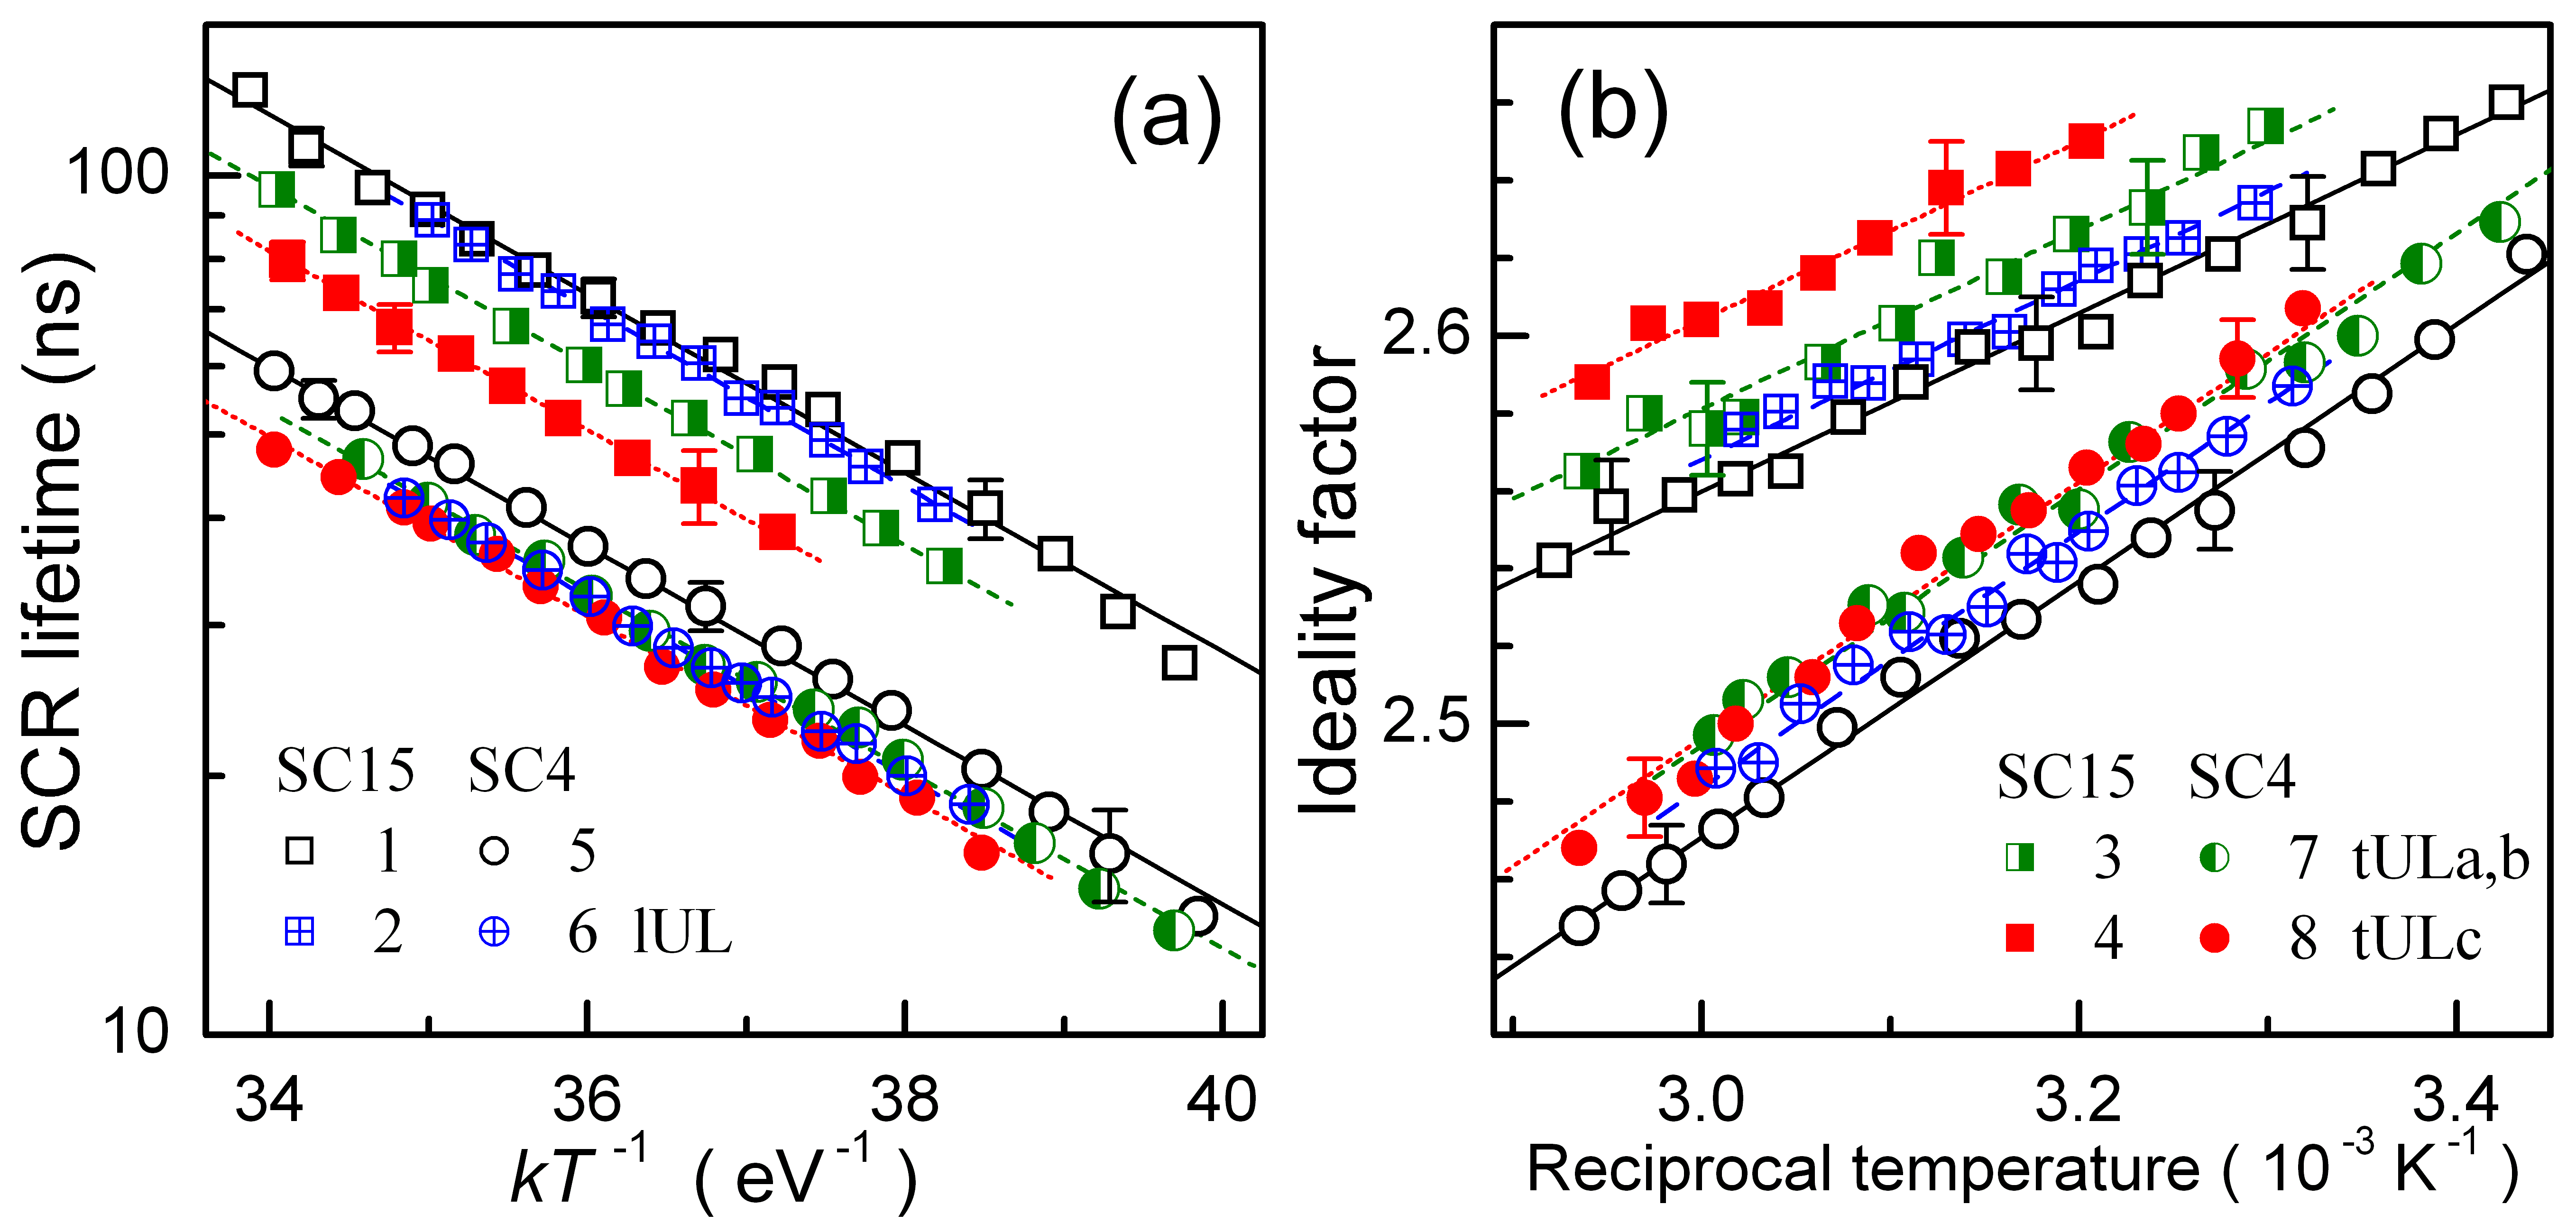
\includegraphics[width=14cm]{olikhFig3}%
\end{center}
\caption{\label{figDUS}
Temperature dependences of SCR carrier lifetime (a) and  ideality factor (b) for SC15 (curves 1--4, squares) and SC4 (5--8, circles).
The curves 1 and 5 (open marks) are obtained without UL,
and  curves 2 and 6 correspond to lUL,
curve 3 corresponds to tULa,
curve 7 corresponds to tULb,
curves 4 and 8 correspond to tULc.
The marks are the experimental results, and the lines are the fitted curves using
Eq.~(\ref{eq_TAUgT}) and $E_{\tau g}=0.24$~eV (a) or
Eq.~(\ref{eq_nT}) and $T_\mathrm{id}=330$ or 230~K (b).
}%
\end{figure}



As seen from Fig.~\ref{figDUS} and Table~\ref{tabParam},
\begin{enumerate}[(i)]
\item UL leads to the increase in $n\mathrm{id}$ and decrease in $\tau_{g}$;
 the AI changes are listed in Table~\ref{tabAIEfect};
\item $\tau_{g}$ and $n\mathrm{id}$ are varied by tUL more effectively;
$\varepsilon_{\tau g}$ and $\Delta n_\mathrm{id}$ increase with $W_{\mathtt{US}}$ enhancement;
\item UL does not affect $E_{\tau g}$ and $T_\mathrm{id}$ values;
$E_{\tau g}$ is equal to $0.24\pm0.01$~eV;
$T_\mathrm{id}$ depends on sample and is equal to $330\pm30$~K (in the SC4 case) or $230\pm20$~K (in the SC15 case).
\end{enumerate}


For the purpose of our analysis, it is important to discuss the recombination mechanism in SCR of the investigated samples.
At first, the large $n_{\mathrm{id}}$ value and small $\tau_g$ value should be accentuated.
According to classical SRH theory, the ideality factor must be smaller than 2, and
$\tau_g$ temperature dependence is expected \cite{TAUg:Schroder,TAUg:Aharoni} to be described by the relation
\begin{equation}
  \tau_g\simeq2\,\tau_n\sqrt{\sigma_n/\sigma_p}\cosh\left[\left(E_t-E_i\right)/kT\right]
\end{equation}
where
$\sigma_n$, $\sigma_p$, and  $E_t$ are the electron and hole capture cross sections (CCSs) and the energy  level of  the  recombination  center,
and $E_i$  is the  intrinsic  energy level.
In our case, $n_{\mathrm{id}}$ is greater than 2, and $\tau_g$ increases with temperature.
Therefore, SRH theory cannot be applied in our case.

Several attempts to account for large $n_\mathrm{id}$ value have been made by using different models.
According to van der Heide \emph{et al.} \cite{Heide}, the nonuniform contact resistance of the front side metallisation leads to a high $n_\mathrm{id}$ value.
However, this theory predicts the dependence of ideality factor on light intensity, whereas $n_\mathrm{id}$ change with $W_{ph}$ is not observed in our case.
Beier and Voss \cite{Beier} explain the large $n_\mathrm{id}$ by the saturation effects within the SRH--model.
However, this theory is unable to explain the $J_{0SCR}$ magnitude, which is much greater than expected for a silicon.
The large ideality factor is attributed to the deep--level--assisted tunneling \cite{Shah,Kaminski_n} too.
But according to this model, the $n_\mathrm{id}$ does not depend on temperature.


At the same time, all the observed features of SCR recombination can be explained by the model of coupled defect level recombination (CDLR) \cite{CDLR:JAP1995,CDLR:JAP,CDLR:SSP}.
According to the CDLR model, the recombination is the result of carrier exchange between two defect levels and crystal bands.
In particular, it is supposed \cite{CDLR:JAP} that the recombination rate is dominant at the sites where acceptor--like defect is coupled with donor-like defect.
In a simplified case, when there is no carrier exchange between the donor level $E_t^{\mathtt{D}}$ and valence band,
as well as between the acceptor level $E_t^{\mathtt{A}}$ and conduction band,
the recombination rate $R$ can be expressed \cite{CDLR:JAP1995} as
\begin{eqnarray}
R&=&\frac{R_{12}-\sqrt{R_{12}^{\,2}-4\tau_{n}^{\mathtt{D}}\tau_{p}^{\mathtt{A}}(np-n_i^2)(1-\epsilon)}}{2\tau_{n}^{\mathtt{D}}\tau_{p}^{\mathtt{A}}(1-\epsilon)}\;,\label{eqR}\\
R_{12}&=&\frac{(n+n_{\mathtt{D}})(p+p_{\mathtt{A}})}{R_{\mathtt{DA}}}+
\tau_{n}^{\mathtt{D}}(p+p_{\mathtt{D}})+\tau_{p}^{\mathtt{A}}(n+n_{\mathtt{A}}),\label{eqR12}\\
\tau_{n}^{\mathtt{D}}&=&(N_{\mathtt{D}}\,\sigma_{n}^{\mathtt{D}}\,\upsilon_{\mathrm{th},n})^{-1},\,\,\,\,
\tau_{p}^{\mathtt{A}}=(N_{\mathtt{A}}\,\sigma_{p}^{\mathtt{A}}\,\upsilon_{\mathrm{th},p})^{-1},\label{eqTAU}
\end{eqnarray}
where
$R_{\mathtt{DA}}$ is the coupling parameter,
$N_{\mathtt{D}}$ and $N_{\mathtt{A}}$ are the densities of donor and acceptor--like defects,
$\sigma_{n}^{\mathtt{D}}$ and $\sigma_{p}^{\mathtt{A}}$ are the electron CCS of the donor and hole CCS of the acceptor,
$\upsilon_{\mathrm{th},n}$ and $\upsilon_{\mathrm{th},p}$ are the thermal electron and hole velocities,
$n_{\mathtt{D,A}}$, $p_{\,\mathtt{D,A}}$, and $\epsilon$ depend on $E_t^{\mathtt{D}}$, $E_t^{\mathtt{A}}$, and level degeneracy  factors.

According to Steingrube \emph{et al}. \cite{CDLR:JAP},
CCS for defect in a pair differs from that for an isolated defect and depends on the distance $r$ between the donor and the acceptor:
\begin{equation}
\label{eqSigma}
\sigma_{n,p}^{\mathtt{D,A}}(r)\propto r^2\,,
\end{equation}
$R_{\mathtt{DA}}$ is proportional to the overlap integral of the defect wave functions as well.
If both defects are characterized by the H--like radial--symmetric wave function and equal Bohr radius $a_0$,
the following expression can be used: \cite{CDLR:JAP}
\begin{equation}
\label{eqRda}
R_{\mathtt{DA}} (r) \propto N_{\mathtt{D}}N_{\mathtt{A}}\left[1+\frac{r}{a_0}+\frac{1}{3}\left(\frac{r}{a_0}\right)^2\right]
   e^{-r/a_0}\,.
\end{equation}


Unfortunately, the equation does not account for the functional relation between $J$--$V$ characteristics parameters and attributes of defects taking part in CDLR.
However, it is shown \cite{CDLR:JAP1995,CDLR:SSP} that $n_{\mathrm{id}}$ increases with the decrement in $R_{\mathtt{DA}}$.
Since $\tau_g\propto R^{-1}$, the $n_{\mathtt{D,A}}$, $p_{\,\mathtt{D,A}}$, and $\epsilon$ are expected to provide a thermoactivated behavior of SCR lifetime.
In our opinion, the value of $E_{\tau g}$ is mainly determined by by couple component energy levels,
whereas the value  of $T_\mathrm{id}$ is affected by $N_\mathtt{D}$ and $N_\mathtt{A}$ too.
Hence,
%data in Fig.~\ref{figDUS} and Table~\ref{tabParam} show that
(i)~same defects are take part in the SCR recombination in both  SC15 and SC4 because the $E_{\tau g}$ values are identical;
(ii)~the defect concentrations in SC15 and SC4 are different because the $T_\mathrm{id}$, $\tau_{g,in}$, and $n_{\mathrm{id},in}$ values
are different;
%the SC4 defect concentration is greater and  donor--acceptor distance is less than those in SC15 because the SC4 $\tau_{g,in}$ and $n_{\mathrm{id},in}$ values are less;
(iii)~UL does not result in the  modification of the level position as well as defect concentration because the $E_{\tau g}$ and $T_\mathrm{id}$ values are not affected.



In our opinion, the observed reversible AI modifications of $n_{\mathrm{id}}$ and $\tau_g$ are induced by
donor--acceptor distance alteration in the samples under UL.
In fact, according to the data \cite{MirzadeJAP2011,PeleshchakUJF2016}, the force acting on a point defect during UL can be expressed as
\begin{equation}
\label{eqFd}
F_d=\chi\,\Delta\Omega_d\frac{\partial \xi(x,t)}{\partial x}\,,
\end{equation}
where
$\chi$ is the bulk elasticity modulus,
$\Delta\Omega_d$ is the crystal volume change per defect
(e.g. $\Delta\Omega_d<0$ and $\Delta\Omega_d>0$ for the vacancy and interstitial atom, respectively),
$\xi$ is the crystal lattice deformation,
and AW propagates along $x$ axis,
$\partial \xi(x,t)/\partial x\propto \xi_{\mathtt{US}}$.
Therefore, a point defect vibrates under UL, so oscillation amplitude and phase are determined by both the defect character and AW intensity.


\begin{figure}
\begin{center}
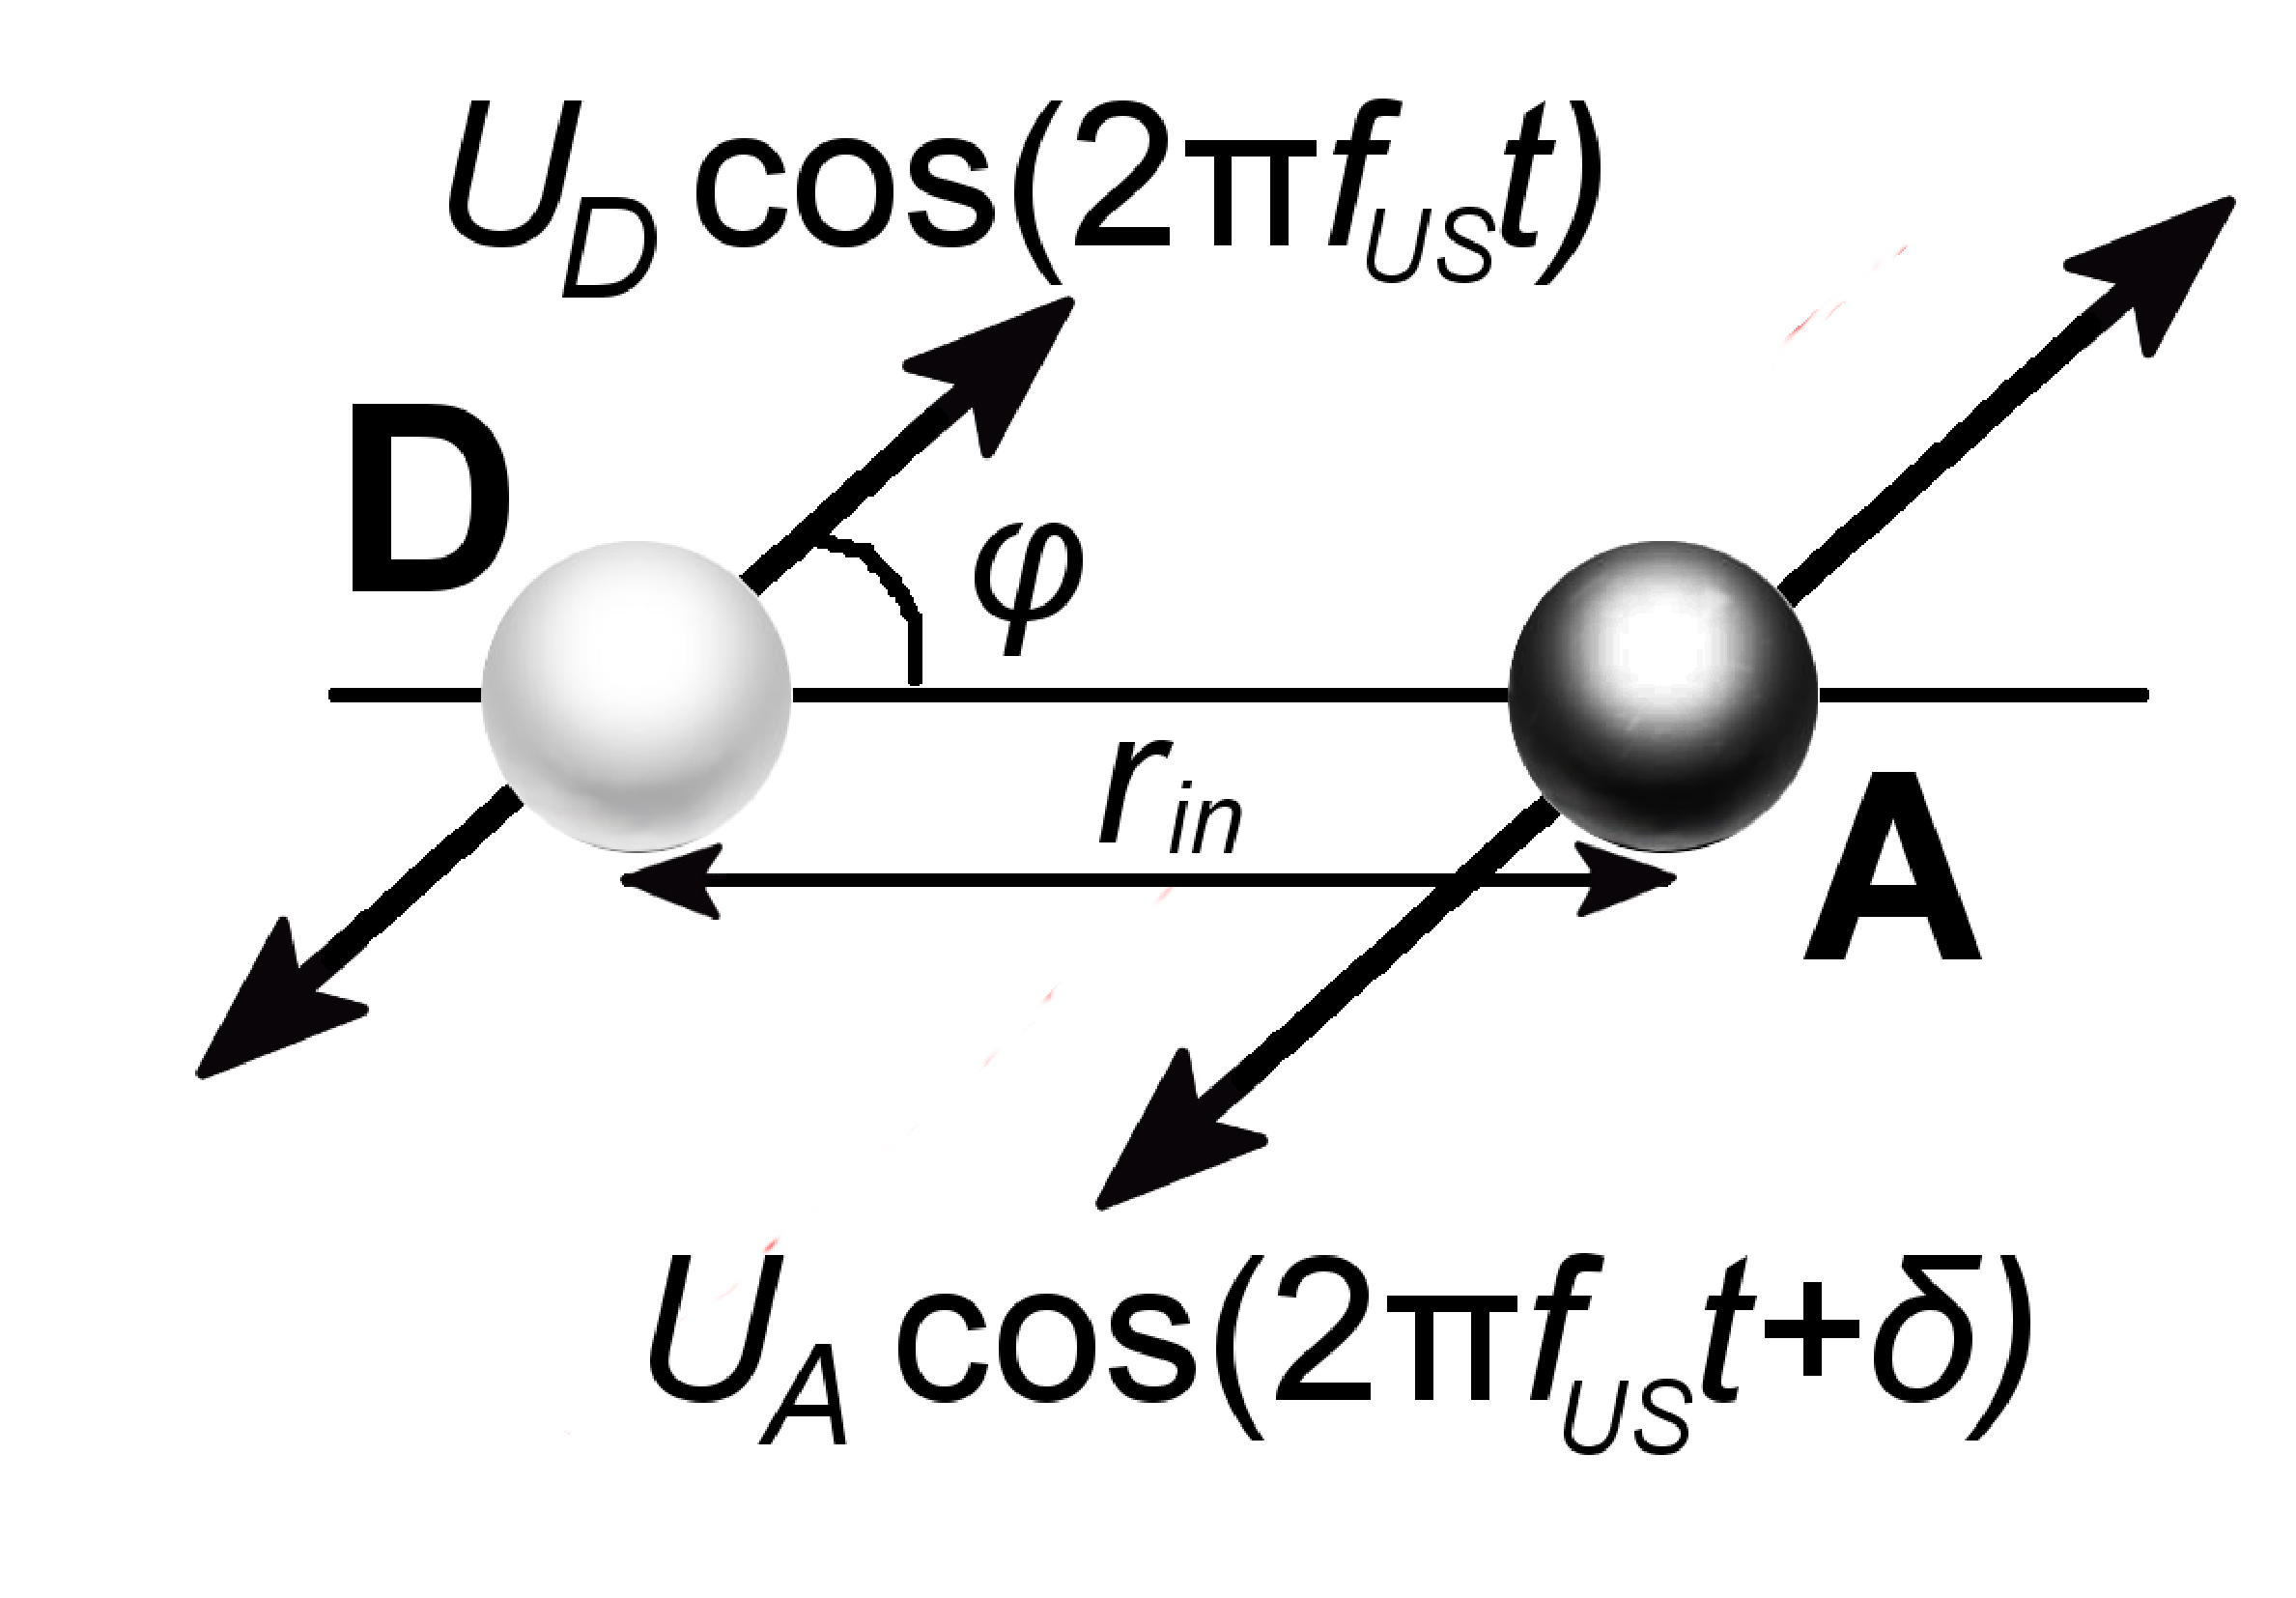
\includegraphics[width=7.5cm]{olikhFig4}%
\end{center}
\caption{\label{figModel}
Model of CDLR center behavior under US action.
}%
\end{figure}

The simplest model, which is shown in Fig.~\ref{figModel}, gives the following  qualitative conclusion.
Initially, the donor (D) and the acceptor (A) are separated by the distance $r_{in}$.
Under UL, the defects would vibrate with amplitudes $u_\mathtt{D}$ and $u_\mathtt{A}$.
Depending on $\xi_{U\!S}$, defect elastic strain ($\Delta\Omega_d^\mathtt{D}$ and $\Delta\Omega_d^\mathtt{A}$), and defect coupling the defect vibration amplitudes can have different values.
The vibration axis coincides with AW displacement direction and forms angle $\varphi$ with  the line, which passes throw the defect initial positions.
$\delta$ is the phase shift between donor and acceptor vibration.


\begin{figure}
\begin{center}
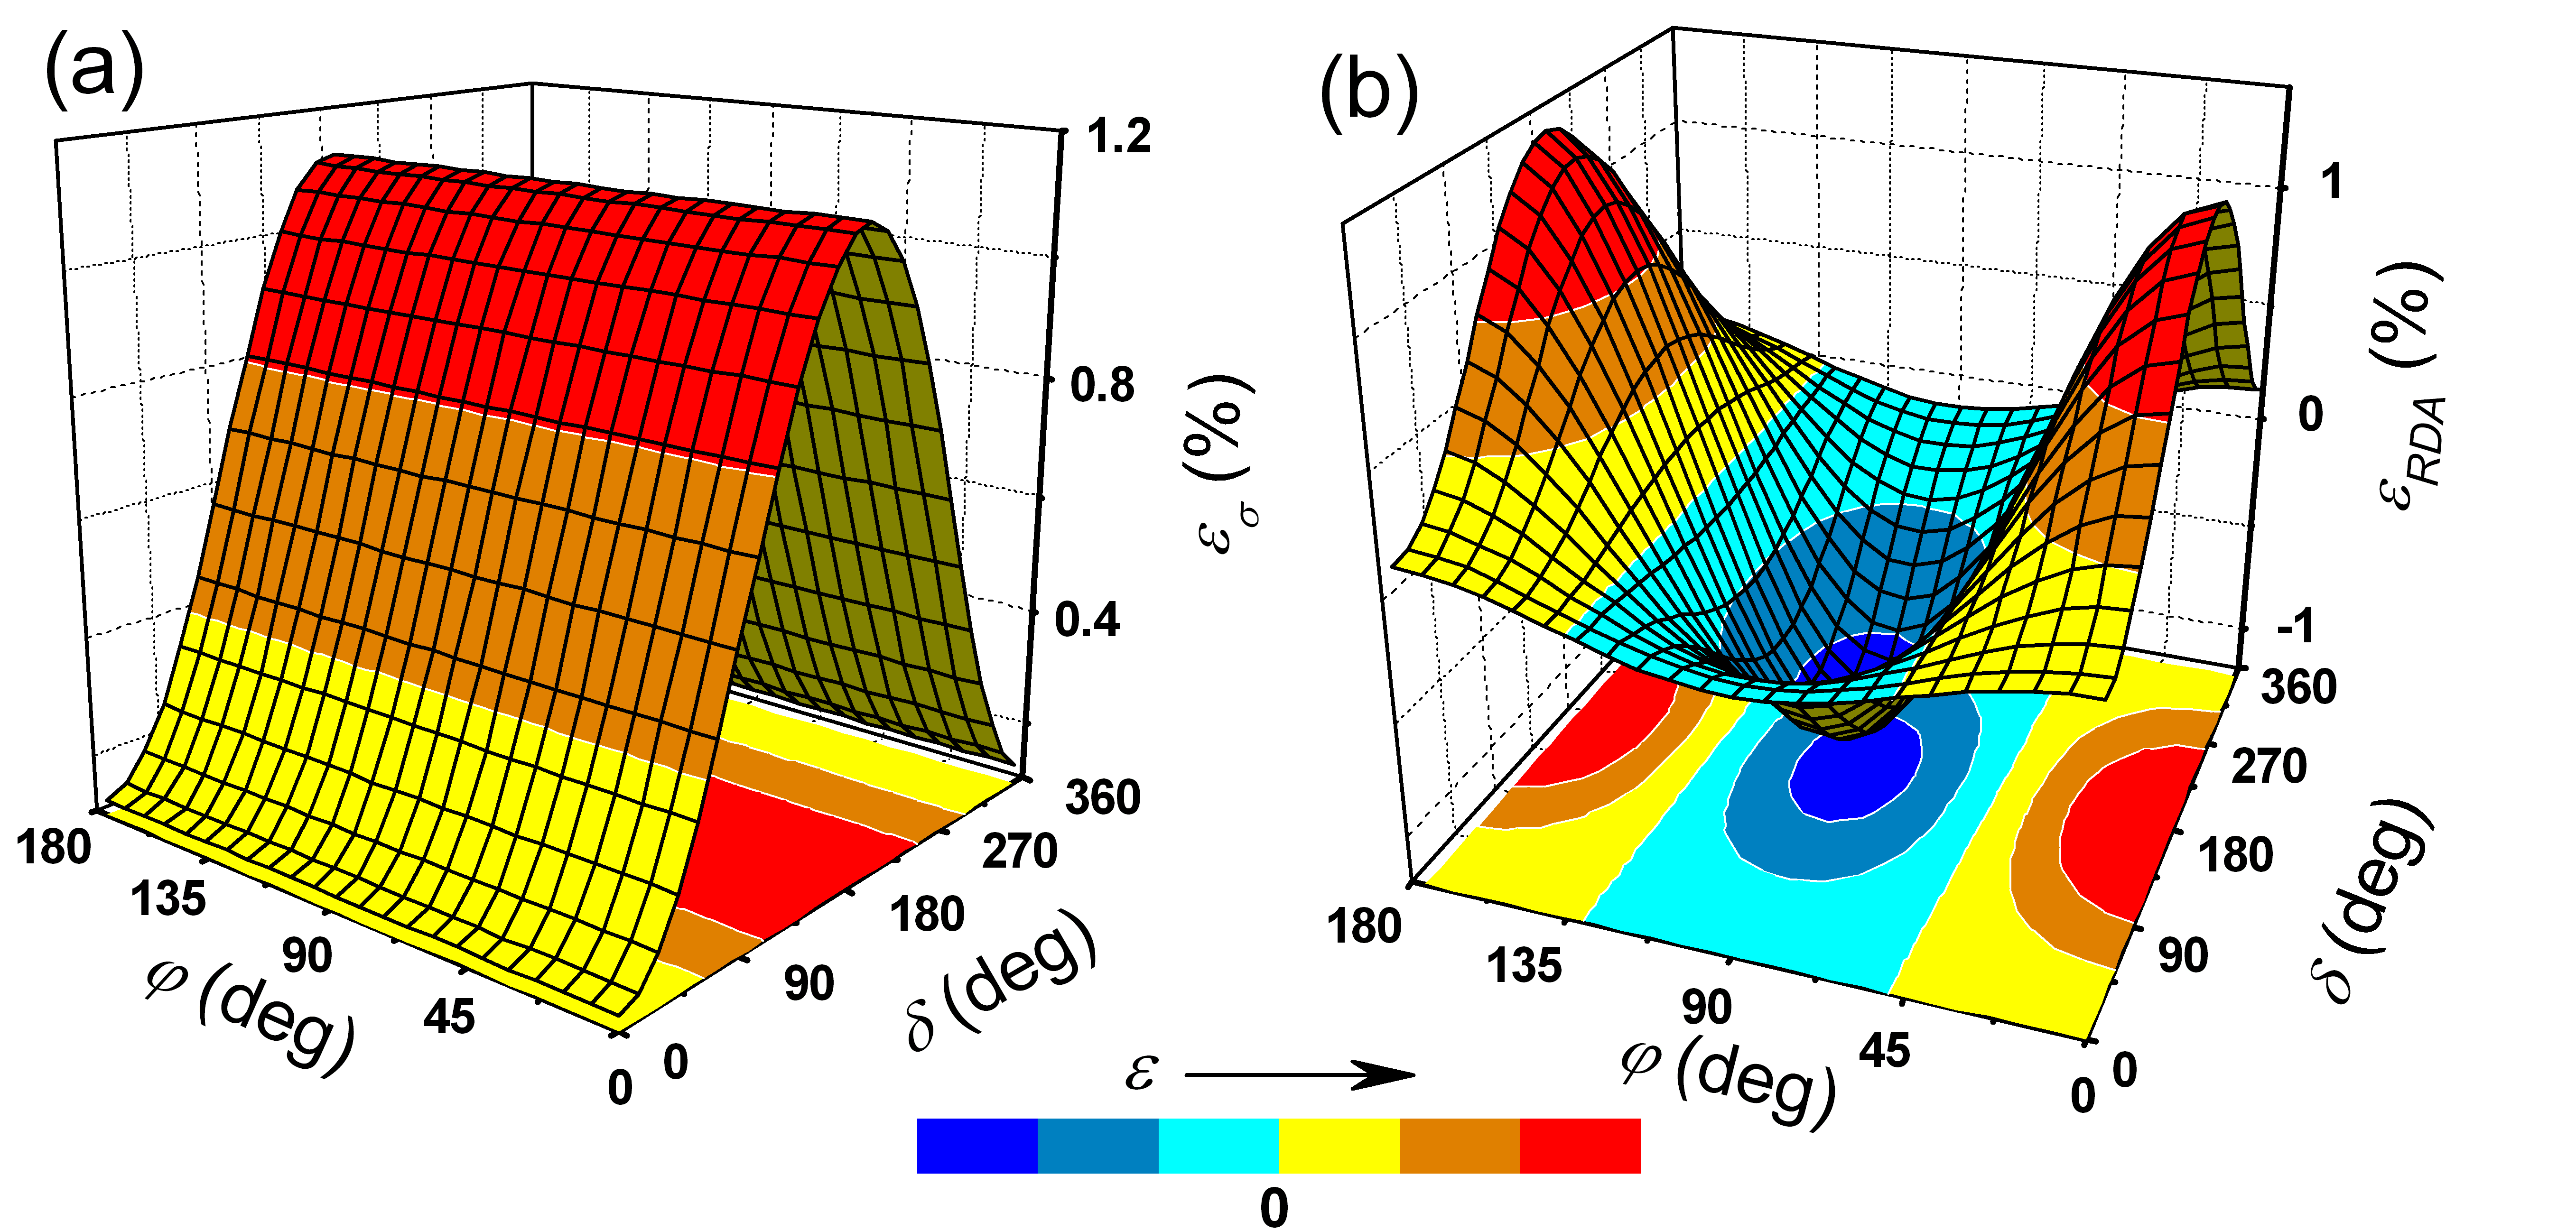
\includegraphics[width=14cm]{olikhFig5}%
\end{center}
\caption{\label{figR2L}
Simulated dependencies of AI changes of capture cross section (a) and coupling parameter (b) on the vibration phase shift  and AW displacement direction.
The parameters are set to $a_0=3.23$~nm, $r_{in}=10$~nm, $u_A=1$~nm, and $u_D=0.5$~nm.
}%
\end{figure}

\begin{figure}
\begin{center}
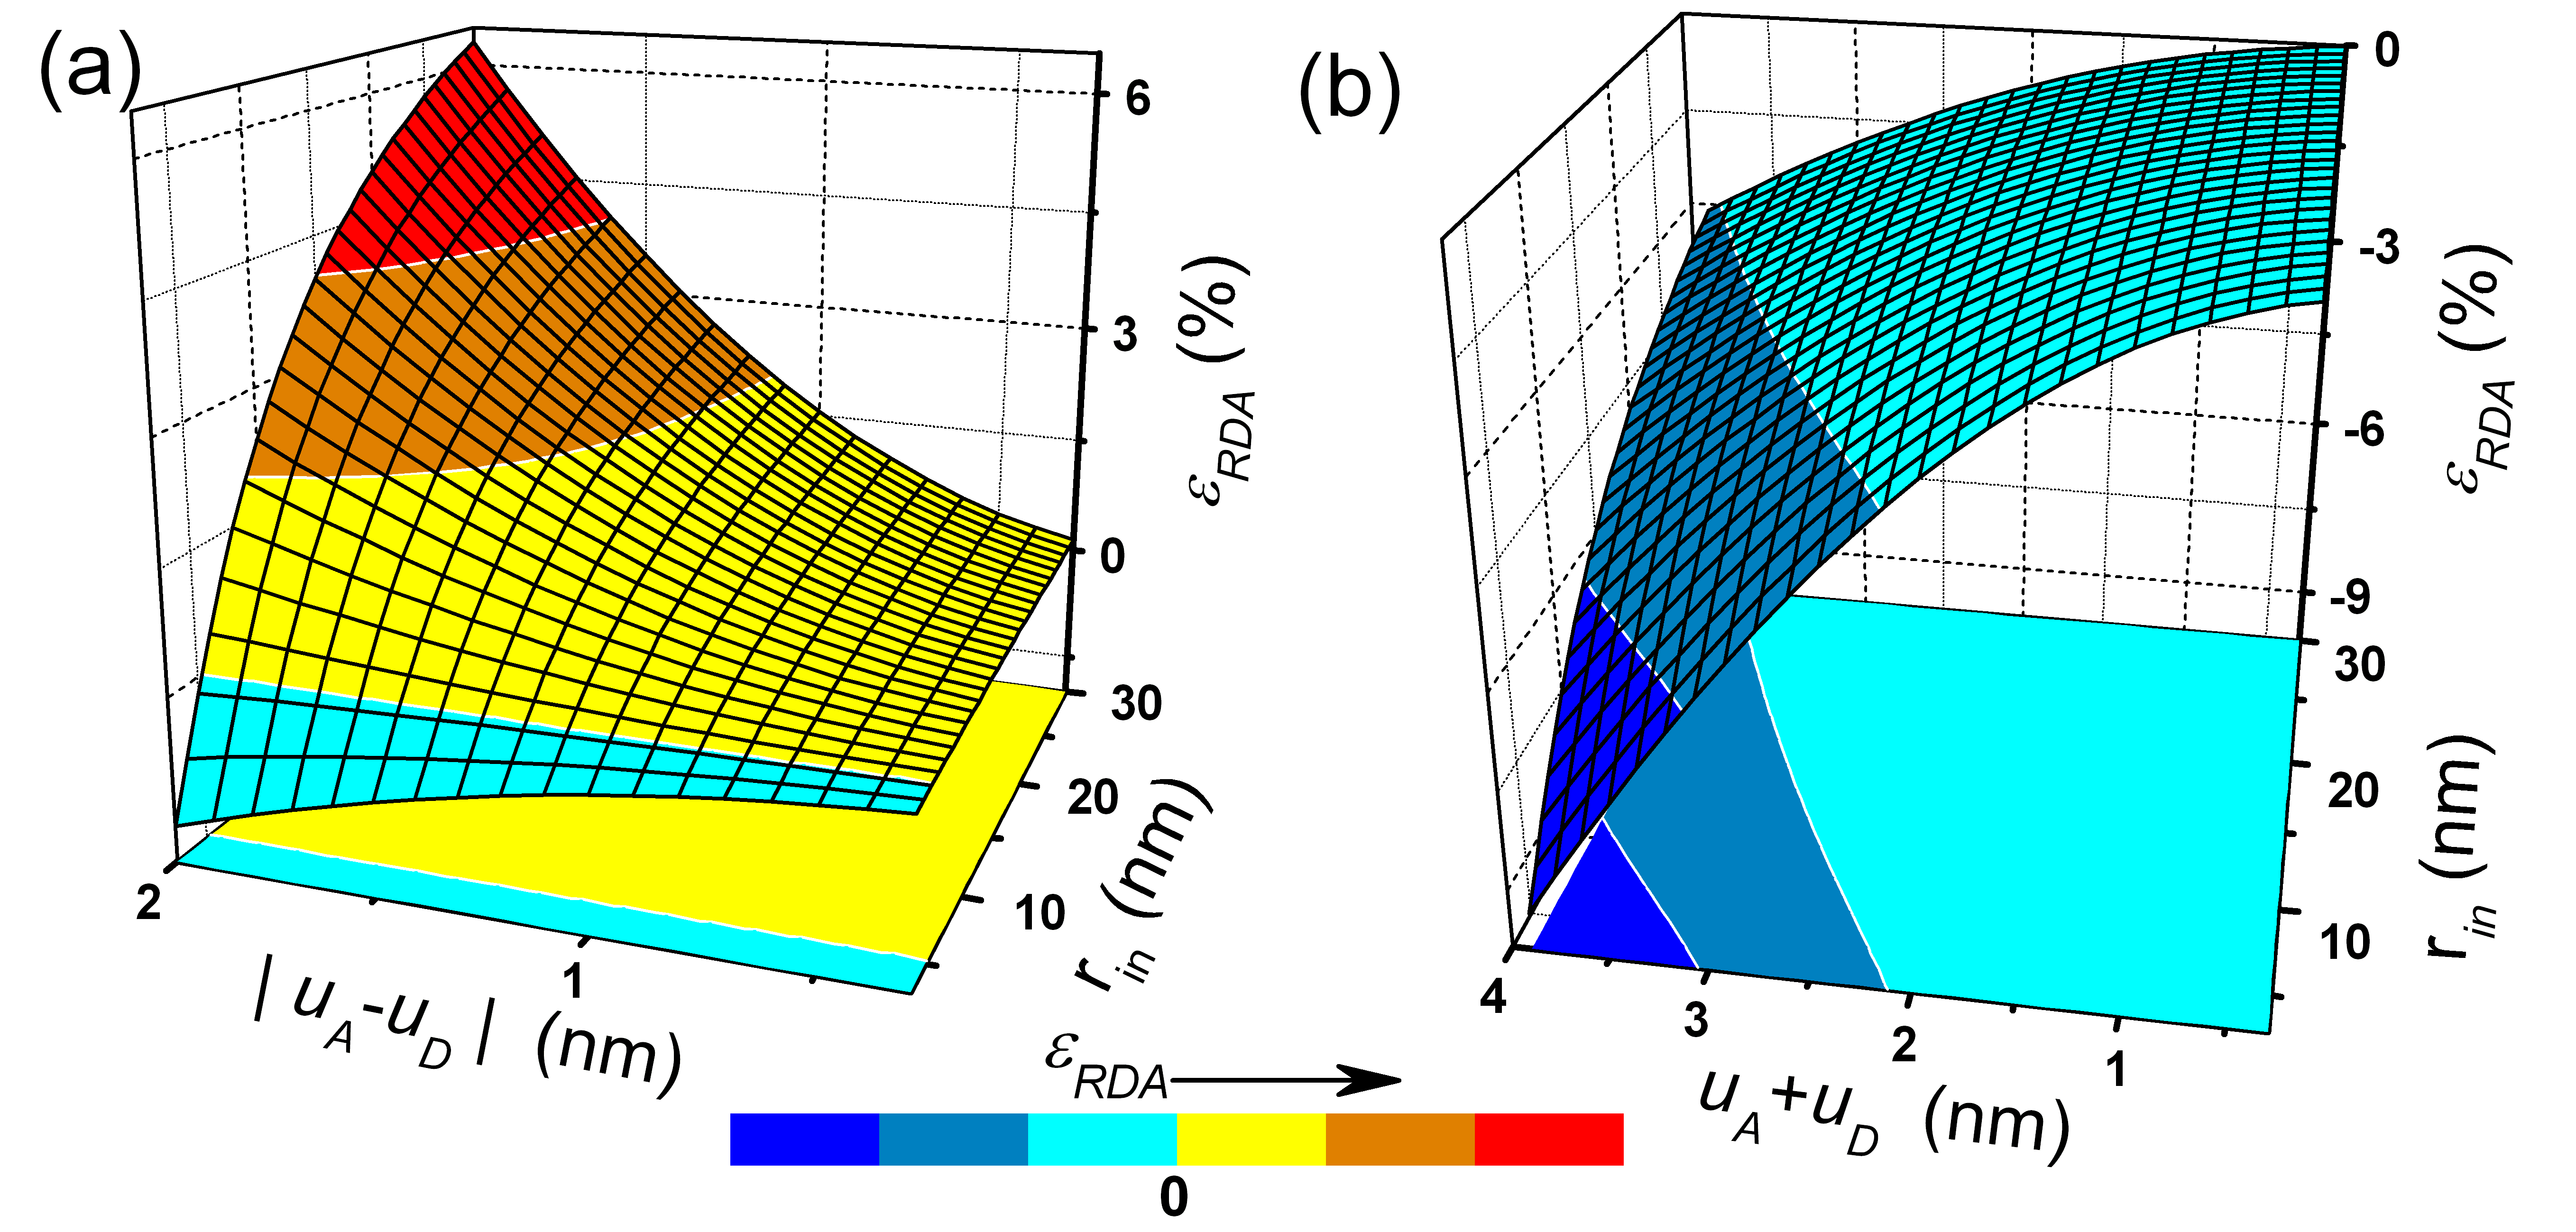
\includegraphics[width=14cm]{olikhFig6}%
\end{center}
\caption{\label{figLnew}
Simulated dependencies of AI changes of coupling parameter on the vibration amplitudes  and initial donor--acceptor distance.
The parameters are set to $\varphi=0^\circ$, $\delta=0^\circ$ (a), and $\varphi=90^\circ$, $\delta=180^\circ$ (b).
}%
\end{figure}

We use Eqs.~(\ref{eqSigma}) and (\ref{eqRda}) to estimate AI relative changes of CCS
$\varepsilon_\sigma=[\sigma_{\mathtt{US}}-\sigma(r_{in})]/\sigma(r_{in})$
and coupling parameters $\varepsilon_{\mathtt{RDA}}=[R_{\mathtt{DA,US}}-R_\mathtt{DA}(r_{in})]/R_\mathtt{DA}(r_{in})$,
where $\sigma_{\mathtt{US}}$ and $R_{\mathtt{DA,US}}$ are averaged over the AW period.
The results of simulation are shown in Figs.~\ref{figR2L} and \ref{figLnew}.
In this estimation, the relaxation time in the CDLR sub--system is assumed to be considerably shorter than $f_\mathtt{US}^{-1}$,
and we apply the previously used \cite{CDLR:JAP} value $a_0=3.23$~nm.
In addition, the chosen $u_\mathtt{D}$ and $u_\mathtt{A}$ values are commensurate with $u_\mathtt{US}$.
However, it should be taken into account that the displacement of the point defect without the covalent bond could exceed a matrix atom displacement.


Fig.~\ref{figR2L}(a) show that the UL leads to the increase in SSC.
The AI alteration of coupling parameter is more complicated --- see Fig.~\ref{figR2L}(b).
In particular, the decrease in $R_{\mathtt{DA}}$ is expected in case of $\varphi\approx90^\circ$ [the couple axis is perpendicular to the AW displacement direction, see Fig.~\ref{figLnew}(b)] or in case of low $r_{in}/a_0$ value [see Fig.~\ref{figLnew}(a)].
In the lat case, the intensive CDLR is expected \cite{CDLR:JAP1995,CDLR:JAP}.
%Besides, simulations show that the US influence increases with decrease in $r_{in}$.

Thus, according to the our model estimation,
UL causes the donor�-acceptor distance change and results in $\varepsilon_{\sigma}$ and $\varepsilon_{\mathtt{RDA}}$,
which mainly depend on lattice deformation.
According to the CDLR theory,  the increase in the SSC and decrease in the coupling parameters should lead to the decrease in the carrier lifetime and increase in the ideality factor.
It was observed in the experiment.


\subsection{Quasi--neutral region \label{P2}}

Base lifetime describes the processes which occur in the quasi--neutral region  of the solar sell.
Fig.~\ref{figDUS_Tau} shows  $\tau_n$  behaviour in the explored temperature range.
As expected, minority carrier lifetime increases as the temperature increases.
The determined by fitting $\tau_n$, calculated $L_n$ values, and its changes are given in  Tables~\ref{tabParam} and \ref{tabAIEfect}.
The obtained values of $L_{n,in}$ are comparable with the $L_{n,in}^{ph}$ values.
The small quantitative difference between the $\varepsilon_{L n}^{ph}$ and $\varepsilon_{L n}$ values, in our opinion, deals with the AI change of the $L_n$ temperature dependence, which is not taken into account during the $J_{sc}(T)$ fitting.


\begin{figure}
\begin{center}

\includegraphics[width=7.5cm]{olikhFig7}%
\end{center}
\caption{\label{figDUS_Tau}
Temperature dependences of base lifetime for SC15 (curves 1--4, squares) and SC4 (5--8, circles).
The curves 1 and 5 (open marks) are obtained without UL,
and  curves 2 and 6 correspond to lUL,
curve 3 corresponds to tULa,
curve 7 corresponds to tULb,
curves 4 and 8 correspond to tULc.
}%
\end{figure}


The calculation shows that the both band--to--band recombination and Auger recombination can be neglected in the investigated samples.
Therefore, the SRH recombination should be only under consideration.
In case of the low injection level, SRH lifetime is described by the following equation
\begin{equation}
\label{eqTAUSHRsum}
\tau_n^{-1}=\sum_i\tau_{n,i}^{-1}=\sum_i N_{d,i}\,\sigma_{n,i}\,\upsilon_{\mathrm{th},n}\,,
\end{equation}
where
$\tau_{n,i}$ characterizes lifetime due to recombination by $i$--th defect,
and $N_{d,i}$ and $\sigma_{n,i}$ are the concentration and electron CCS of $i$--th defect, respectively.

Fig.~\ref{figDUS_Tau} shows that UL results in a decrease in $\tau_n$.
As AI changes are reversible, the lifetime alteration, in our opinion, deals with the increase in $\sigma_n$ under US action.
The majority of recombination center in the silicon are known to be a complex point defect and a complex components are not the same.
Following the empirical relation  proposed in \cite{CDLR:R2}, we assume that Eq.~(\ref{eqSigma})
is valid for a complex point defect as well.
In this case, however, $r$ is the distance which separates the components of a complex.
According to the model suggested in Sec.~\ref{SCR}, UL leads to $r$ variation.
In the case of CDLR, AI change of the capture cross section of donor (or/and acceptor) is supplemental to the variation of
both the coupling parameter and the couple distance,
but only CCS change determines the AI variation of base lifetime.
If no US  absorption by the defect is assumed, $\delta$ is equal to $0^\circ$ if $(\Delta\Omega_d^\mathtt{D}\cdot\Delta\Omega_d^\mathtt{A})>0$
or to $180^\circ$ if $(\Delta\Omega_d^\mathtt{D}\cdot\Delta\Omega_d^\mathtt{A})<0$.
In this simple case, relative changes of CCS depend on oscillation amplitudes and
do not depend on $\varphi$:
\begin{equation}
\label{eqEpsSig}
\varepsilon_{\sigma}=(u_\mathtt{D}\pm u_\mathtt{A})^2/2\,r_{in}^2\,,
\end{equation}
where``$+$'' and ``$-$'' correspond to $\delta=180^\circ$ and $\delta=0^\circ$, respectively.

The defects in silicon structures are not all acoustically active (AA) and can remain unmodified under the action of ultrasound.
The acousto�defect interaction efficiency depends on the defect type and structure. \cite{UST:Medvid,Olikh2018JAP}.
If only one AA center with $N_{d}^\mathtt{AA}$ and $\sigma_{n}^\mathtt{AA}$ is present in the sample,
Eq.~(\ref{eqTAUSHRsum}) for $\tau_{n}^{-1}$ under UL takes the following shape:
\begin{equation}
\label{eqMS_Us}
\tau_{n,\mathtt{US}}^{-1}=\tau_{n,in}^{-1}+ \varepsilon_{\sigma}N_{d}^\mathtt{AA}\,\sigma_{n}^\mathtt{AA}\,\upsilon_{\mathrm{th},n}=
                          \tau_{n,in}^{-1}+K_\mathtt{US}u_\mathtt{US}^2 \,,
\end{equation}
where
$K_\mathtt{US}$ characterizes the complex--ultrasound interaction and depends on properties defects as well as crystal matrix;
in particular, $K_\mathtt{US}\propto N_{d}^\mathtt{AA}$.
Equation~(\ref{eqMS_Us}) takes into account that $u_\mathtt{D},u_\mathtt{A}\propto \xi_\mathtt{US}\propto u_\mathtt{US}$.
Eq.~(\ref{eqMS_Us}) is similar to the well--known Messenger�-Spratt equation \cite{Markvart}, which describes the irradiation--induced decrease in the lifetime.

The obtained dependences of the reciprocal base lifetime versus the AI atom
displacements are shown in Fig.~\ref{fig_Kus}.
The linearity of these dependences proves the correctness of our assumptions.
The obtained $K_\mathtt{US}$ values are listed in Table~\ref{tabParam}.
The greater $K_\mathtt{US}$ value in SC15 is evident that the AA defect concentration is greater as well.


\begin{figure}
\begin{center}
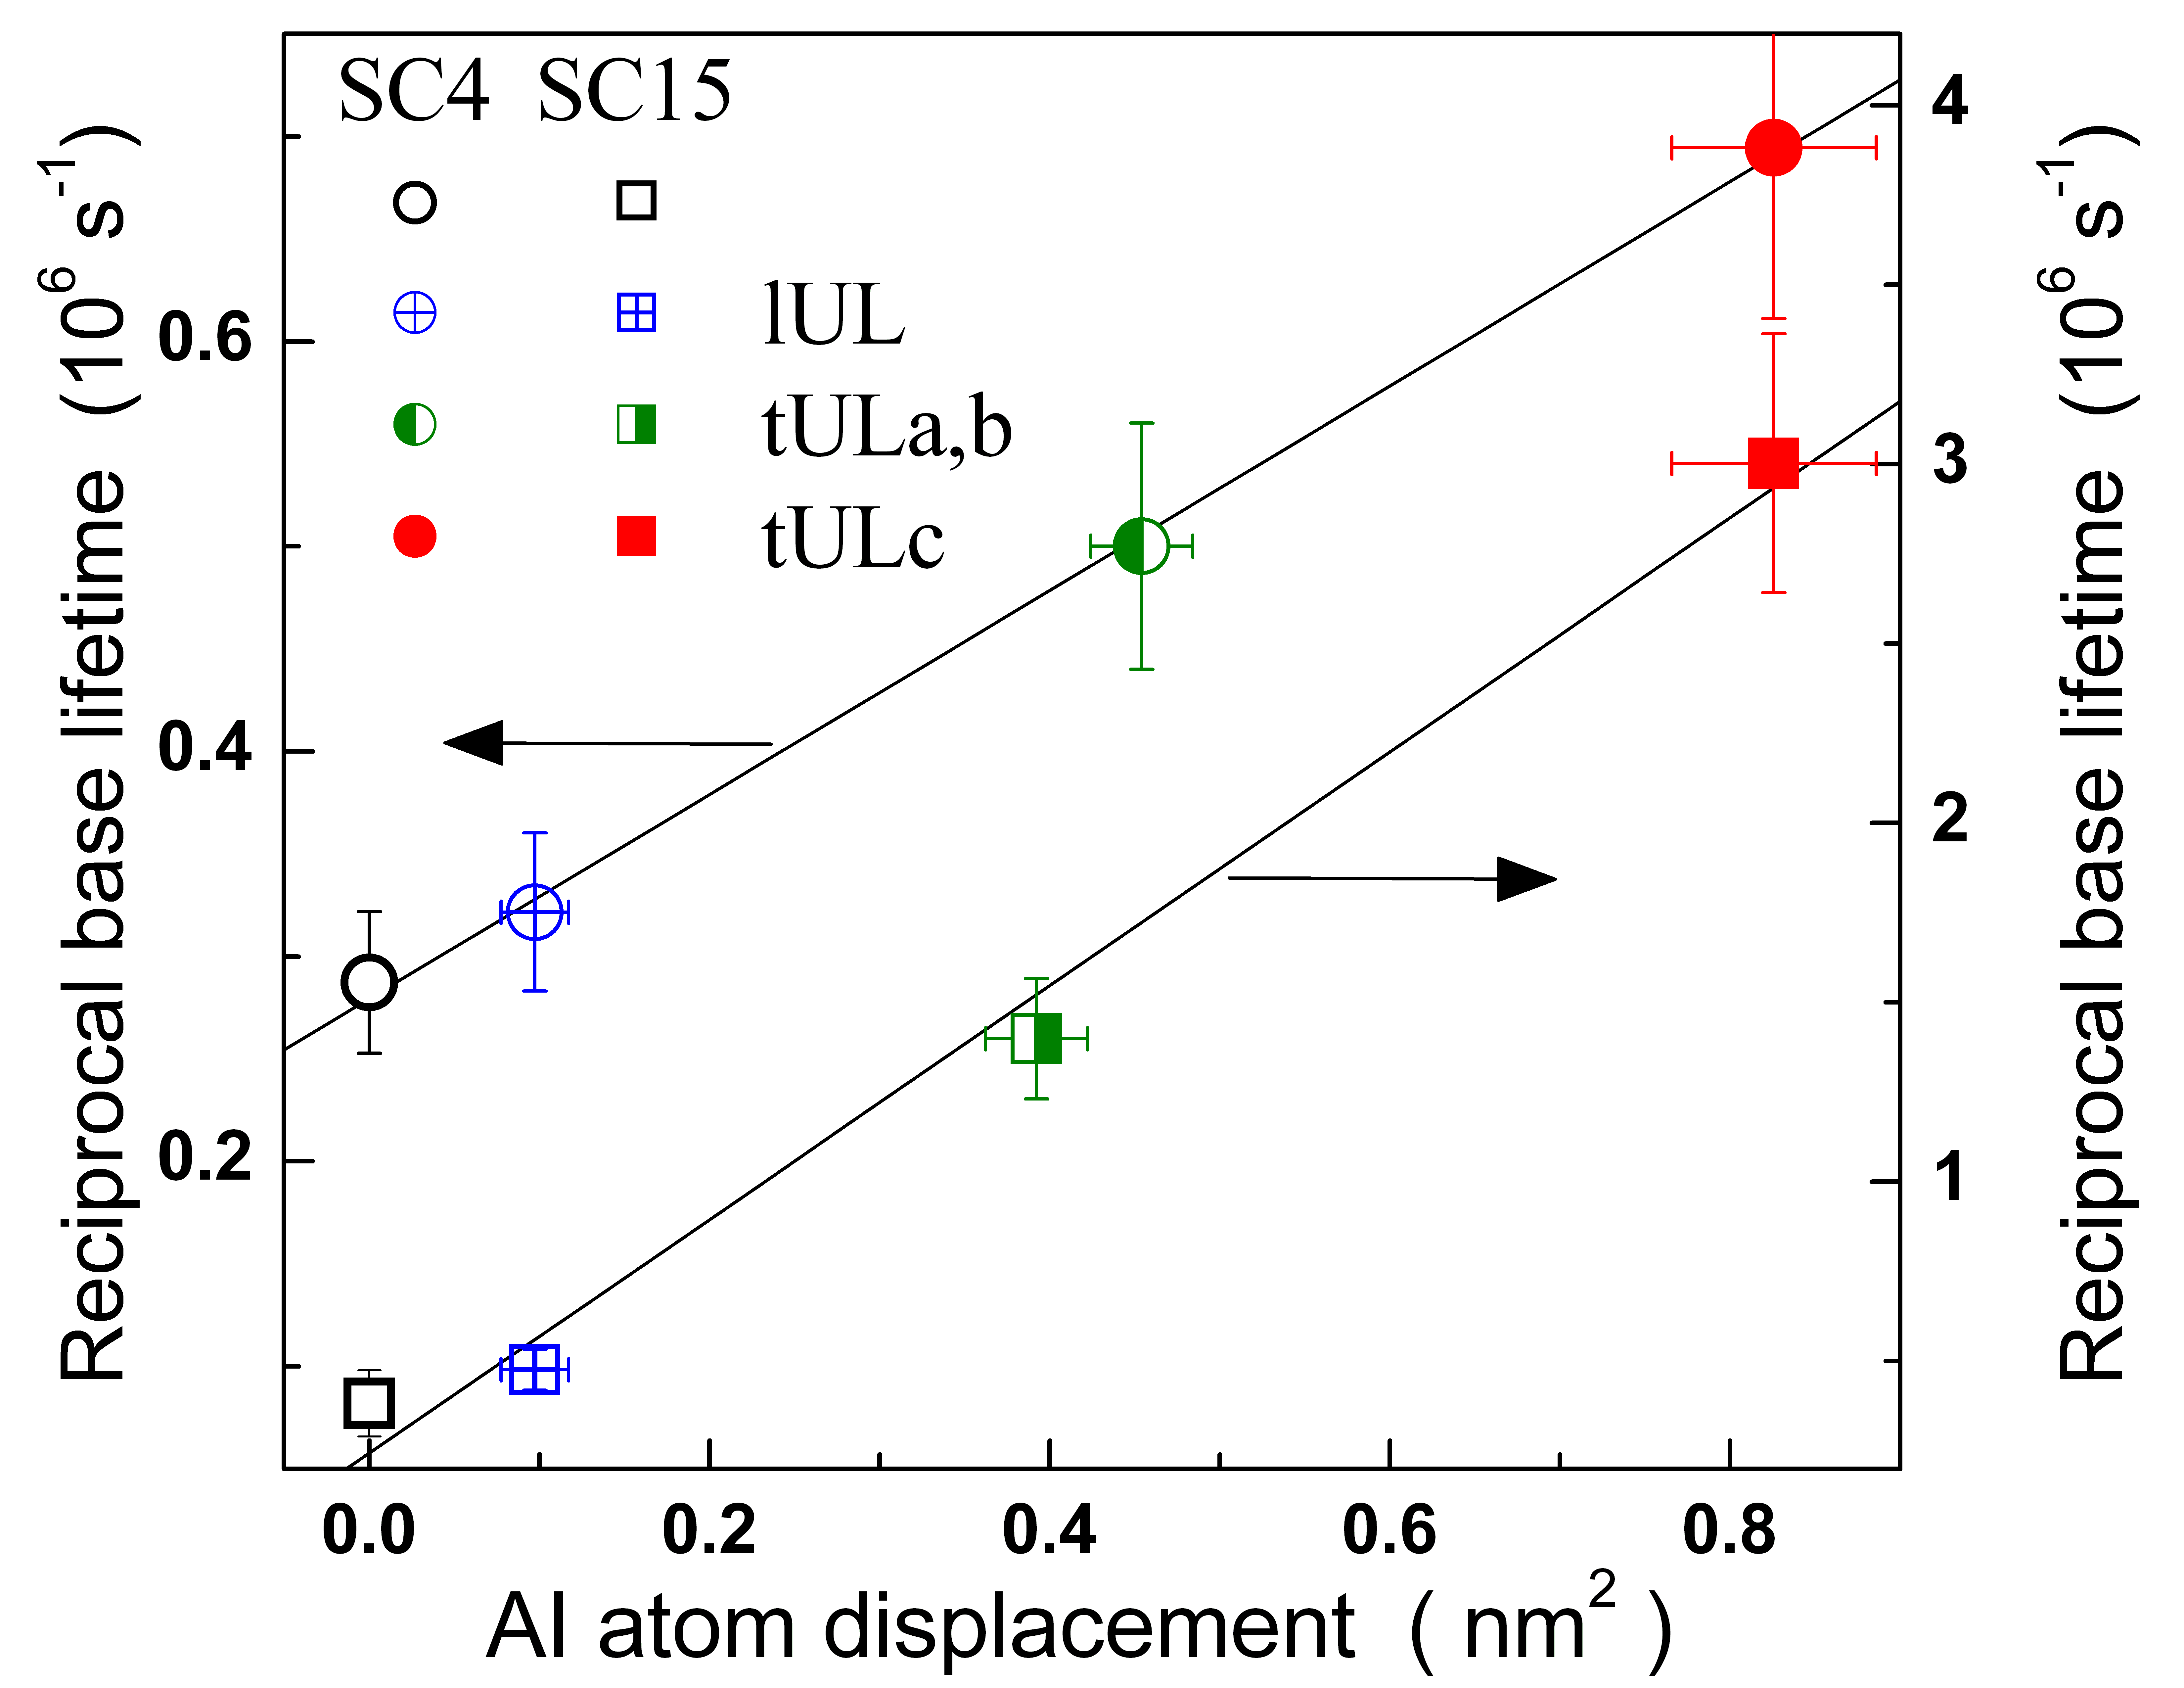
\includegraphics[width=7.5cm]{olikhFig8}%
\end{center}
\caption{\label{fig_Kus}
Dependencies of reciprocal base lifetime on AI lattice atom displacement  for SC15 (squares, right axis) and SCR4 (circles, left axis)at 320~K.
Symbol filling is determined by the AW intensity and type and coincides with Fig.~\ref{figDUS_Tau} notation.
Lines are linear fitting.
}%
\end{figure}


It should be noted that an initial distance between the recombination complex components is much less than the donor--acceptor distance in CDLR.
Therefore, according to Eq.~(\ref{eqEpsSig}), the more effective US influence is expected in the first case and $\varepsilon_{\tau n}>\varepsilon_{\tau g}$ is observed experimentaly.


\subsection{Shunt resistance}

\begin{figure}
\begin{center}
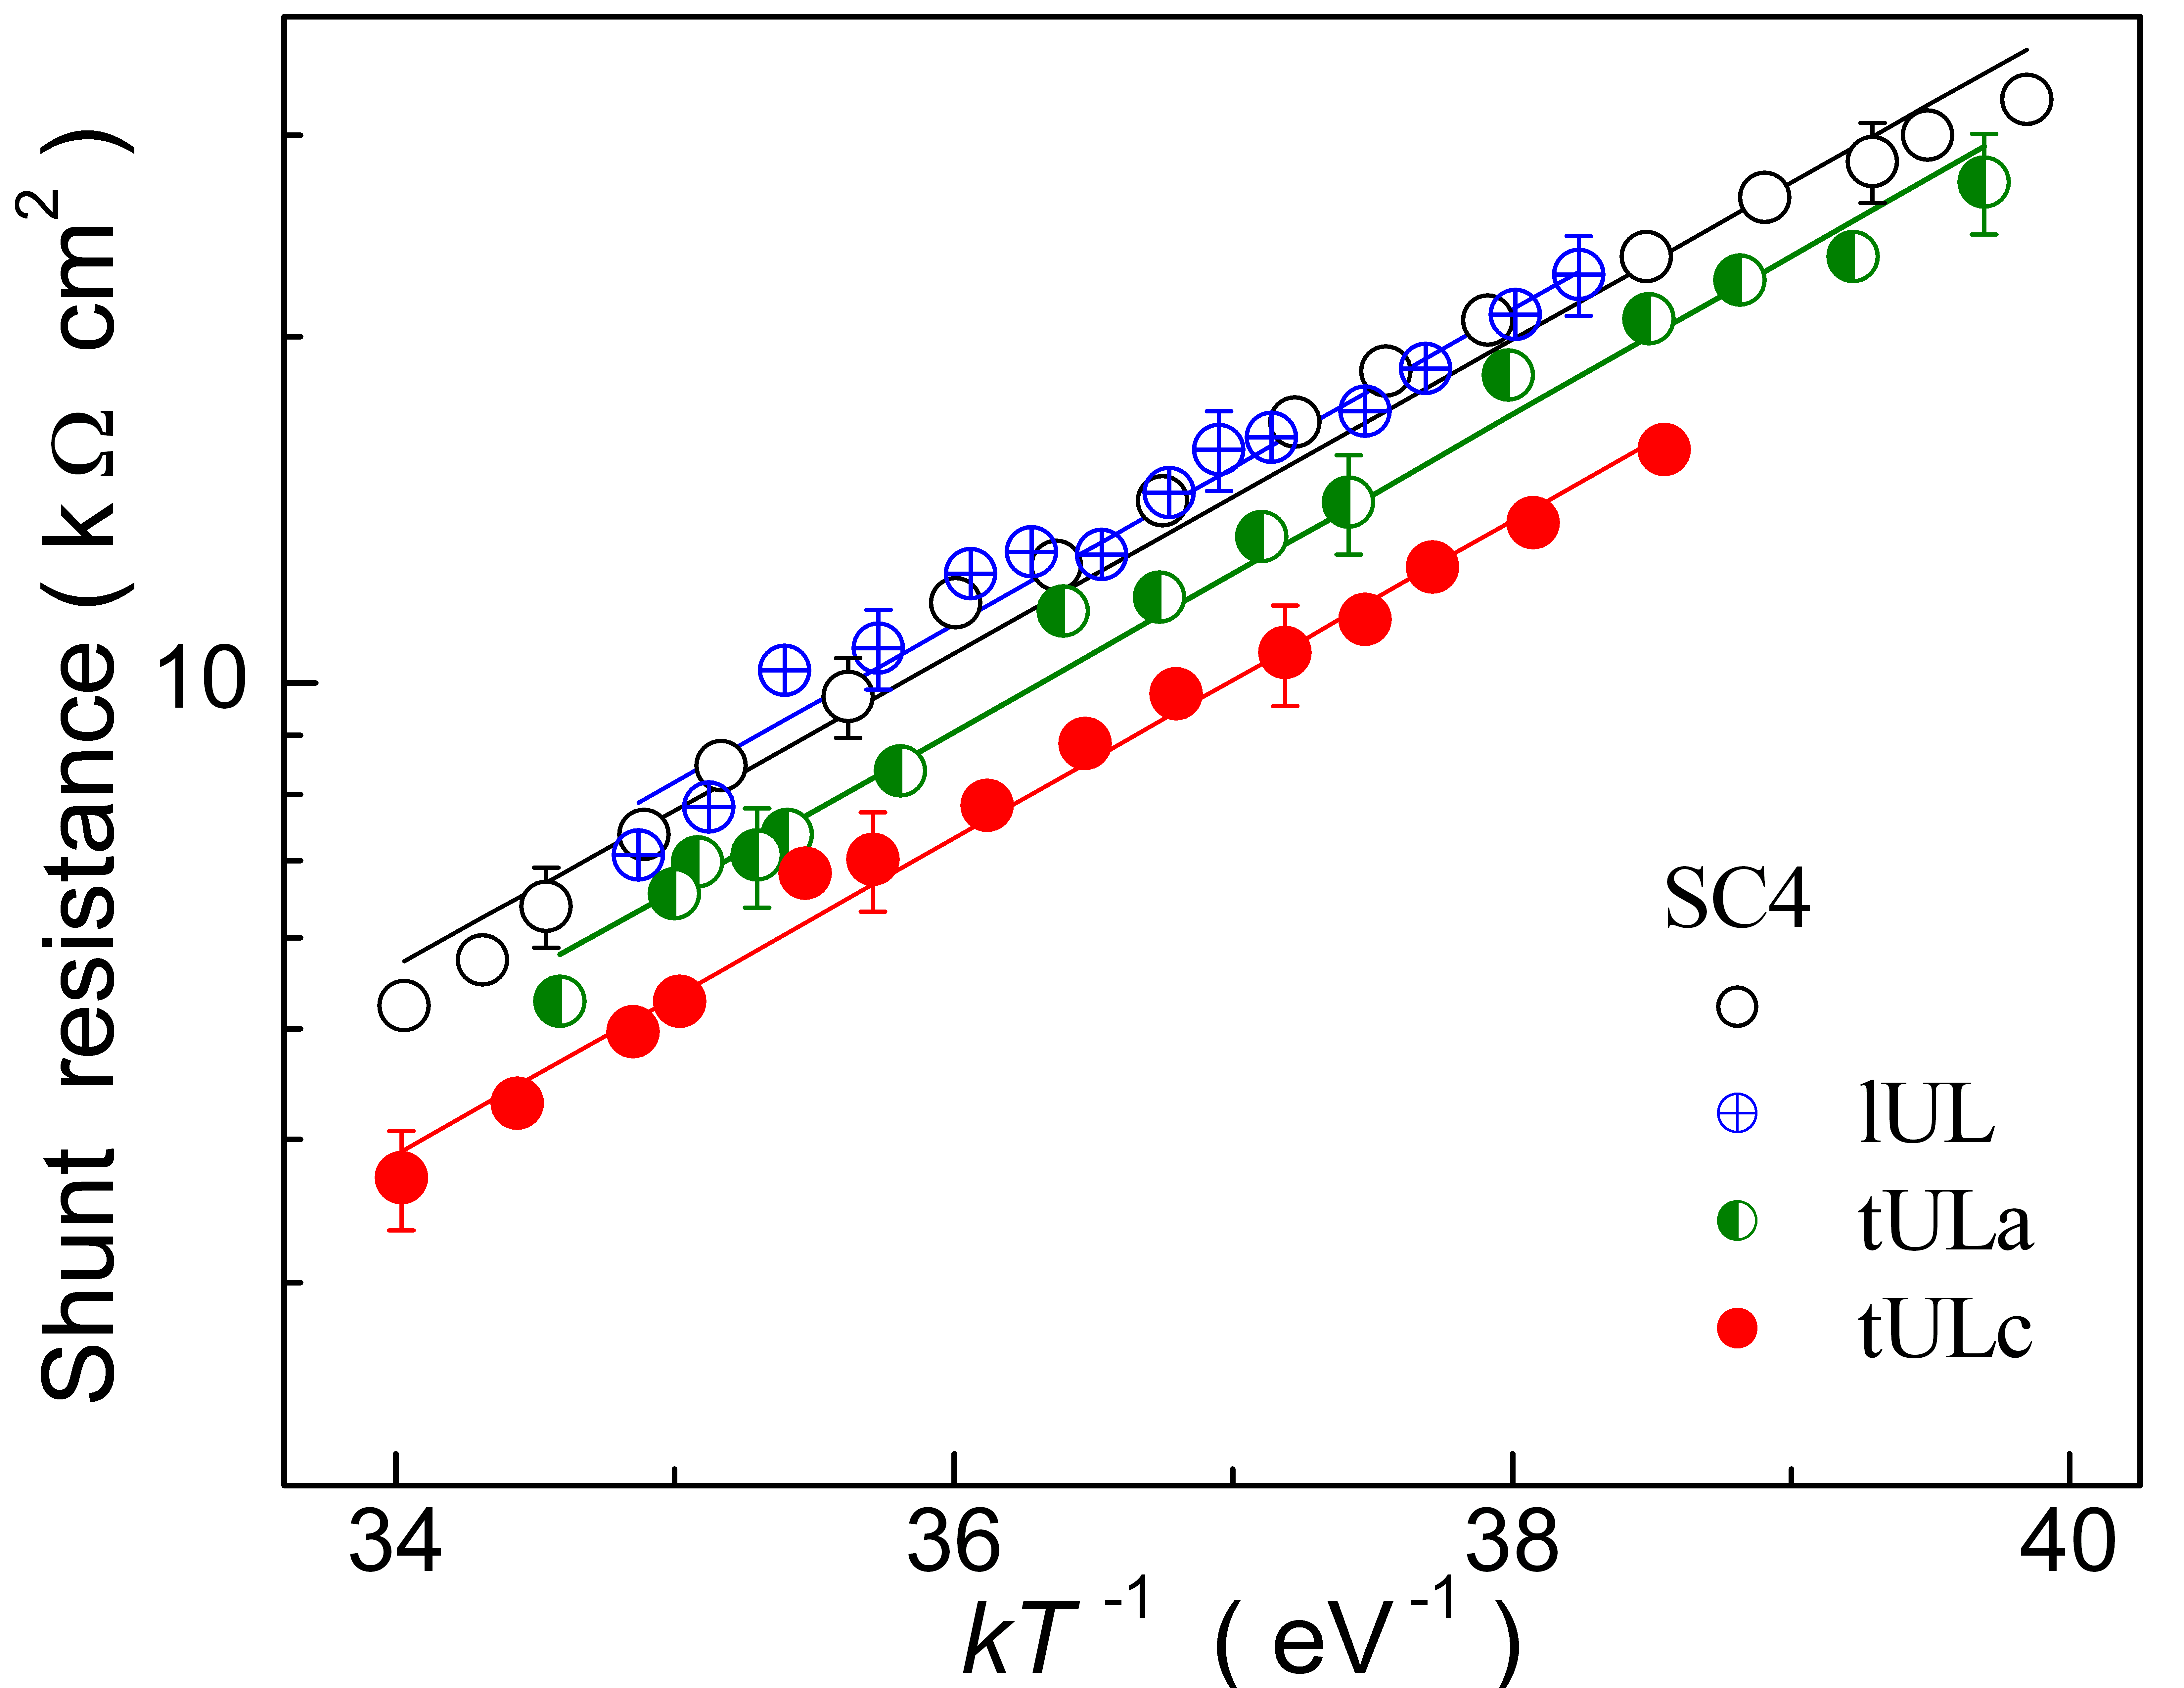
\includegraphics[width=7.5cm]{olikhFig9}%
\end{center}
\caption{\label{figDUS_Rsh}
Temperature dependences of shunt resistance for SC4, obtained with and without (open marks) UL.
%$W_{U\!S}$,W/cm$^2$: 0.18 (2), 0.22 (3), 0.40 (4).
The marks are the experimental results, and the lines are the fitted curves using Eq.~(\ref{eqRsh})
}%
\end{figure}

Fig.~\ref{figDUS_Rsh} shows the  shunt resistance  over the explored temperature range.
As seen from the figure, the tUS results in a decrease in $R_{sh}$ whereas the lUL does not change shunt resistance practically.
The calculated data are listed in Tables~\ref{tabParam} and \ref{tabAIEfect}.

The shunt resistance is known\cite{Rsh:Breitenstein} to occur in $p$--$n$ structure due to several non--mechanical reasons.
It can be caused by aluminum particles, macroscopic Si$_3$N$_4$ inclusions, or inversion layers at precipitates.
In the course of firing, the Al particle can penetrate into the sample creating $p^+$--doped region around it, which compensates the emitter and remains in ohmic contact with the base.
Subsequent annealing should decrease $R_{sh}$,
but this expected behavior  conflicts with data, which are presented therein after, in Sec.~\ref{P3}.
Inversion layers and Si$_3$N$_4$ inclusions occur mainly in multicrystalline silicon cells \cite{Rsh:Breitenstein} and cannot cause shunt resistance in the investigated samples.
Dislocations, however, which intersect the junction, are generally held responsible as a possible source of ohmic current.\cite{Rsh:Breitenstein,TAT:Gopal,Rsh:Baker}
Dislocations should be strongly recombinative, its recombination current may become strong enough for it to act as a shunt.
For this reason they should be decorated by impurities \cite{Rsh:Breitenstein}.


According to the model of dislocation--induced impedance of photovoltaic detector suggested by Gopal and Gupta,\cite{Rsh:Gopal2003,Rsh:Gopal2004}
$R_{sh}$ can be given by:
\begin{equation}
\label{eqRsh}
R_{sh}=\frac{T}{\sigma_{\mathtt{dis}}}\left[\cosh\left(\frac{E_\mathtt{dis}-E_i}{kT}\right)+\cosh\left(\frac{U_s}{kT}\right)\right]\,,
\end{equation}
with
\begin{equation}
\label{eqRdis}
\sigma_{\mathtt{dis}}=\rho_{\mathtt{dis}}A^2q^2A_{\mathtt{dis}}\sqrt{K_nK_p}\,N_{\mathtt{dis}}(n_p+p_p)/k\,,
\end{equation}
where
$E_{\mathtt{dis}}$ is the energy level which significantly contributes to the dislocation recombination current,
$U_s$ is the potential at the surface of the dislocation core,
$A$ is the sample area,
$\rho_{\mathtt{dis}}$ and $A_{\mathtt{dis}}$ are the dislocation density and surface area, respectively,
$K_n$ and $K_p$ are the probabilities for electrons and holes capture by the dislocation states,
and $N_{\mathtt{dis}}$ is the density of surface states at each dislocation.
Equation~(\ref{eqRsh}) is true for the simplified case of $K_p=K_n$.
It should be noted that a similar temperature dependence of a SSC shunt resistance is used elsewhere \cite{RshT} too.


To fit the experimental data for $R_{sh}$, we used Eq.~(\ref{eqRsh}).
As the fitting parameters, $(E_{\mathtt{dis}}-E_i)$, $U_s$, and $\sigma_{\mathtt{dis}}$ were taken.
It has been found that the experimental data are in good agreement with the fitting curves (see Fig.~\ref{figDUS_Rsh}) for values $(E_{\mathtt{dis}}-E_i)=(0.34\pm0.02)$~eV and $U_s=(5\pm4)\times10^{-8}$~eV, which were independent of UL.
The obtained value of $(E_{\mathtt{dis}}-E_i)$ corresponds to the carrier activation energy $0.22\pm0.02$~eV and
is comparable with the
$0.22\div0.25$~eV \cite{Edis:Evans}, $0.28$~eV \cite{Edis:Castaldini}, $0.19$~eV \cite{Edis:Omling}, and $0.23$~eV \cite{Edis:Ogawa},
which was earlier reported for an impurity at the dislocation or with an intrinsic dislocation level.

tUL causes  $\sigma_{\mathtt{dis}}$ increase.
In our opinion, this is caused by an $A_\mathtt{dis}$ augmentation.
Namely, the dislocation core atom displacement  is  parallel or normal to the  current direction in case of lUL or tUL, respectively.
As a result, the carriers are captured by dislocation levels from enlarged volume in the tUL case.
Therefore, the effective surface area increases and $R_{sh}$ decreases due to US action.


\subsection{Open--circuit voltage and fill factor simulation\label{P4}}


In order to visualize  dependencies of the open--circuit voltage and fill factor on $\tau_n$, $n_\mathrm{id}$, $\tau_g$, and $R_{sh}$, the following procedure was used.
Firstly, we used Eqs.~(\ref{eqIV})--(\ref{eqIph}) to  simulated $J$--$V$ characteristics taking the various values of $\tau_g$, $\tau_n$, $n_{\mathrm{id}}$, and $R_{sh}$.
The parameters values, which are close to those of investigated SSCs, are used in simulation.
Secondly, $V_{oc}$ and $F\!F$ were estimated from the obtained $J$--$V$ curves by the conventional mode.
The results are shown in Figures \ref{figVoc} and \ref{figFF}.


\begin{figure}
\begin{center}
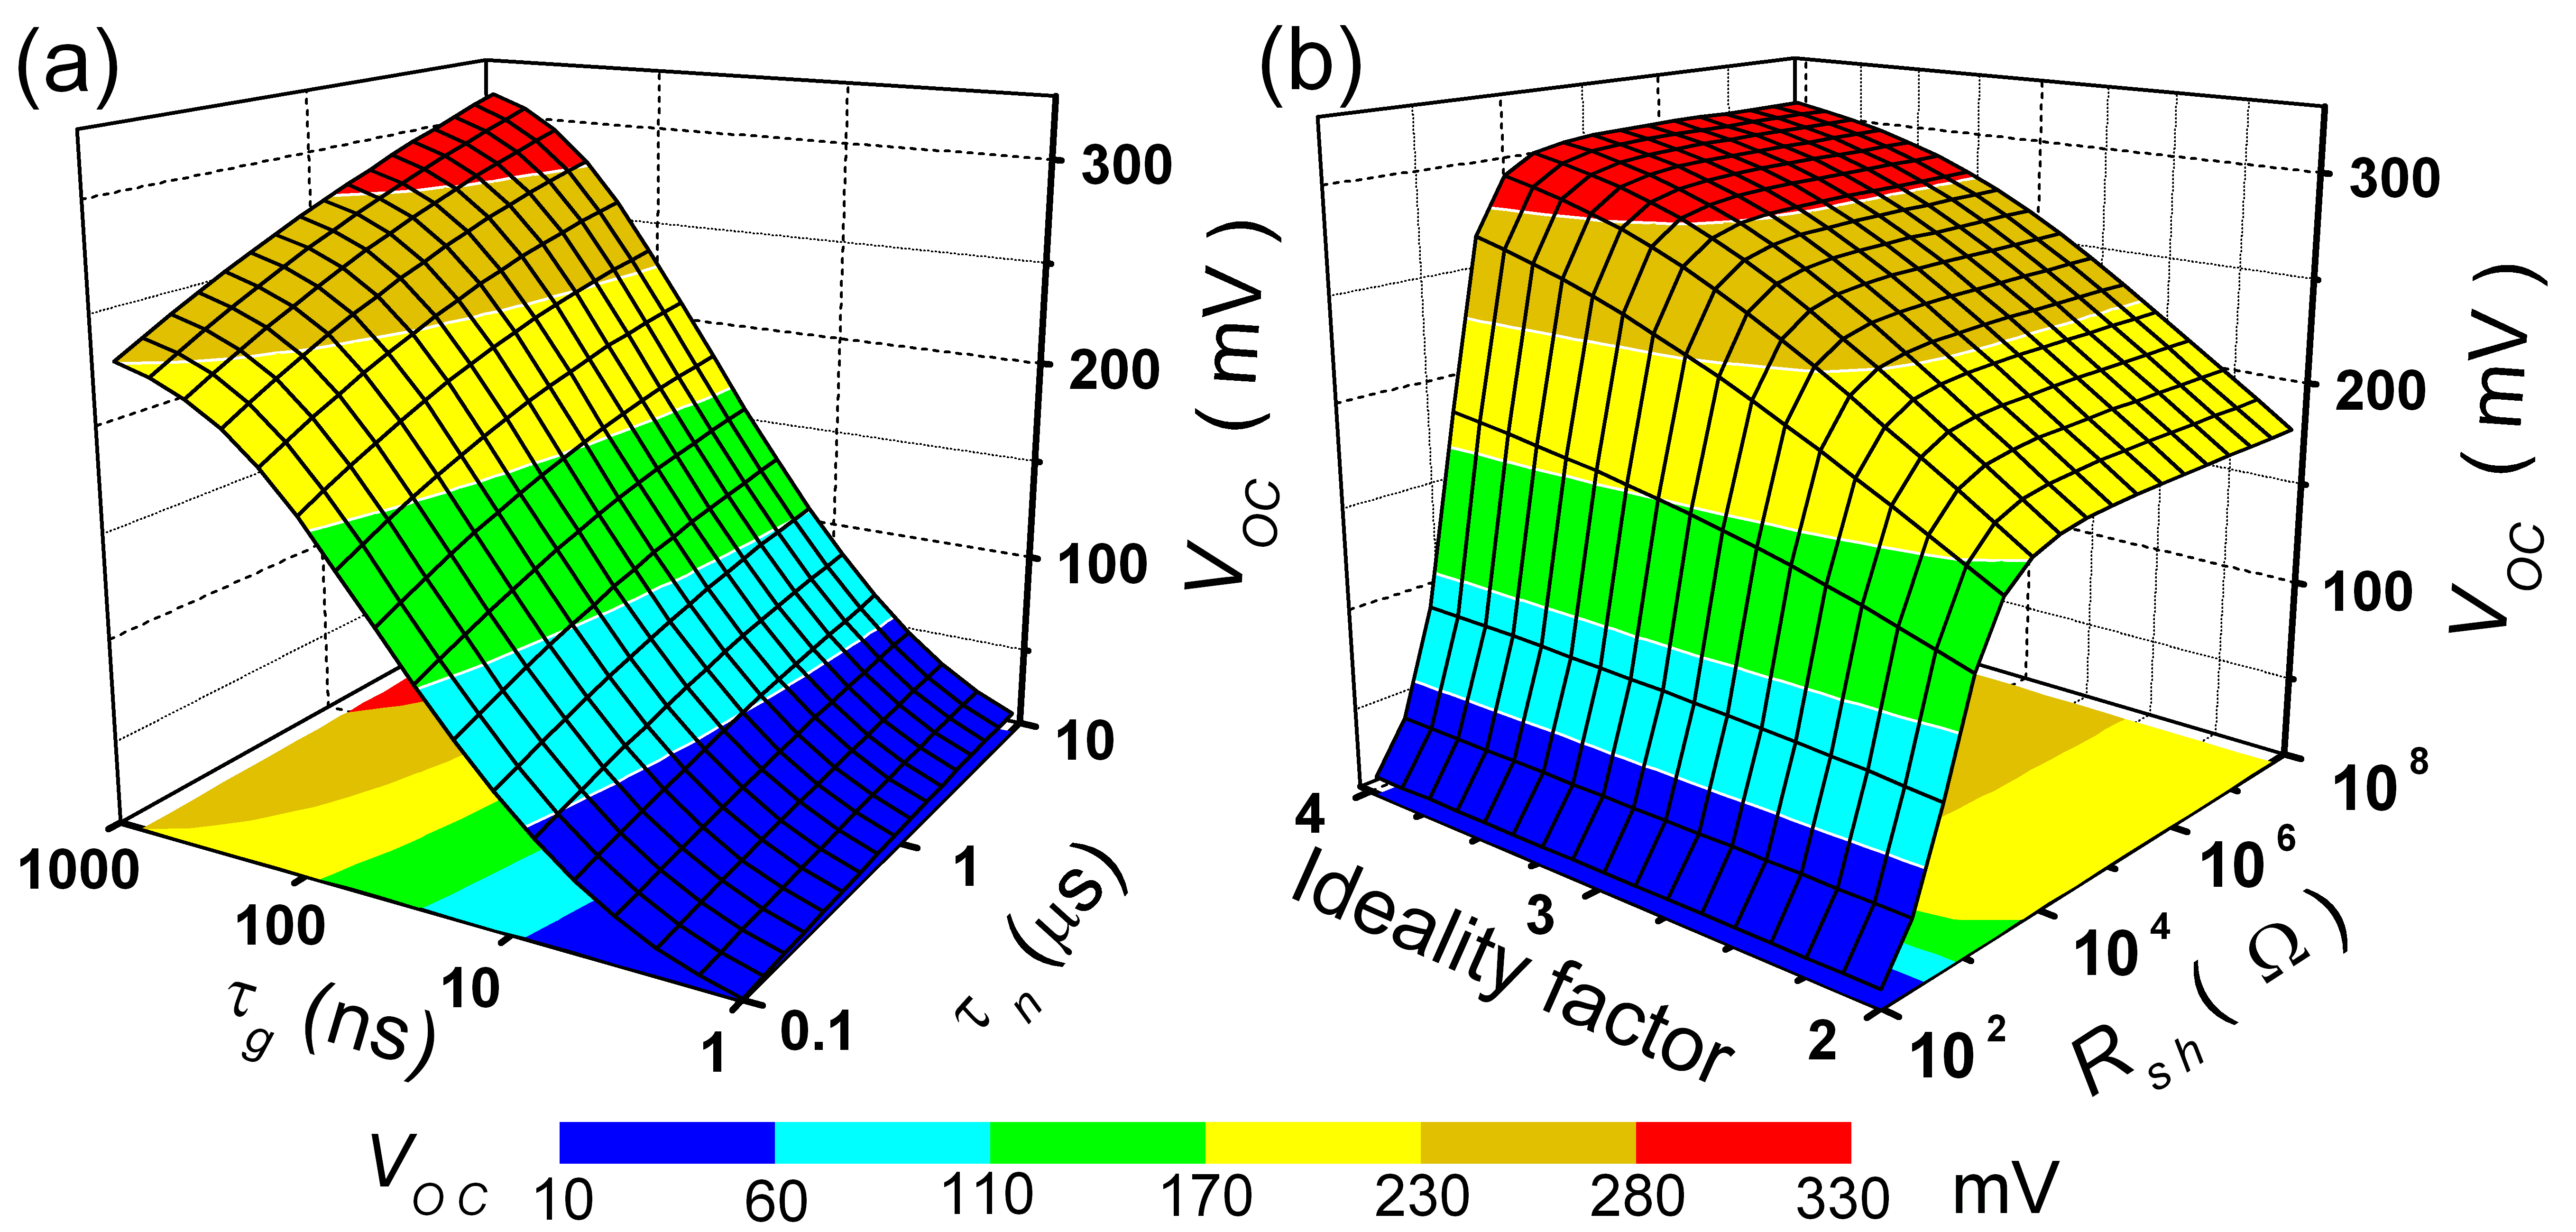
\includegraphics[width=14cm]{olikhFig10}%
\end{center}
\caption{\label{figVoc}
Simulated open--circuit voltage dependencies on the SCR lifetime and base lifetime (a), and on the ideality factor and shunt resistance (b).
The constant values $n=2.55$ (a), $R_{sh}=5\times10^3$~$\Omega$ (a), $\tau_n=3\times10^{-6}$~s (b), $\tau_g=5\times10^{-8}$~s (b), and $T=320$~K were used.
}%
\end{figure}


\begin{figure}
\begin{center}
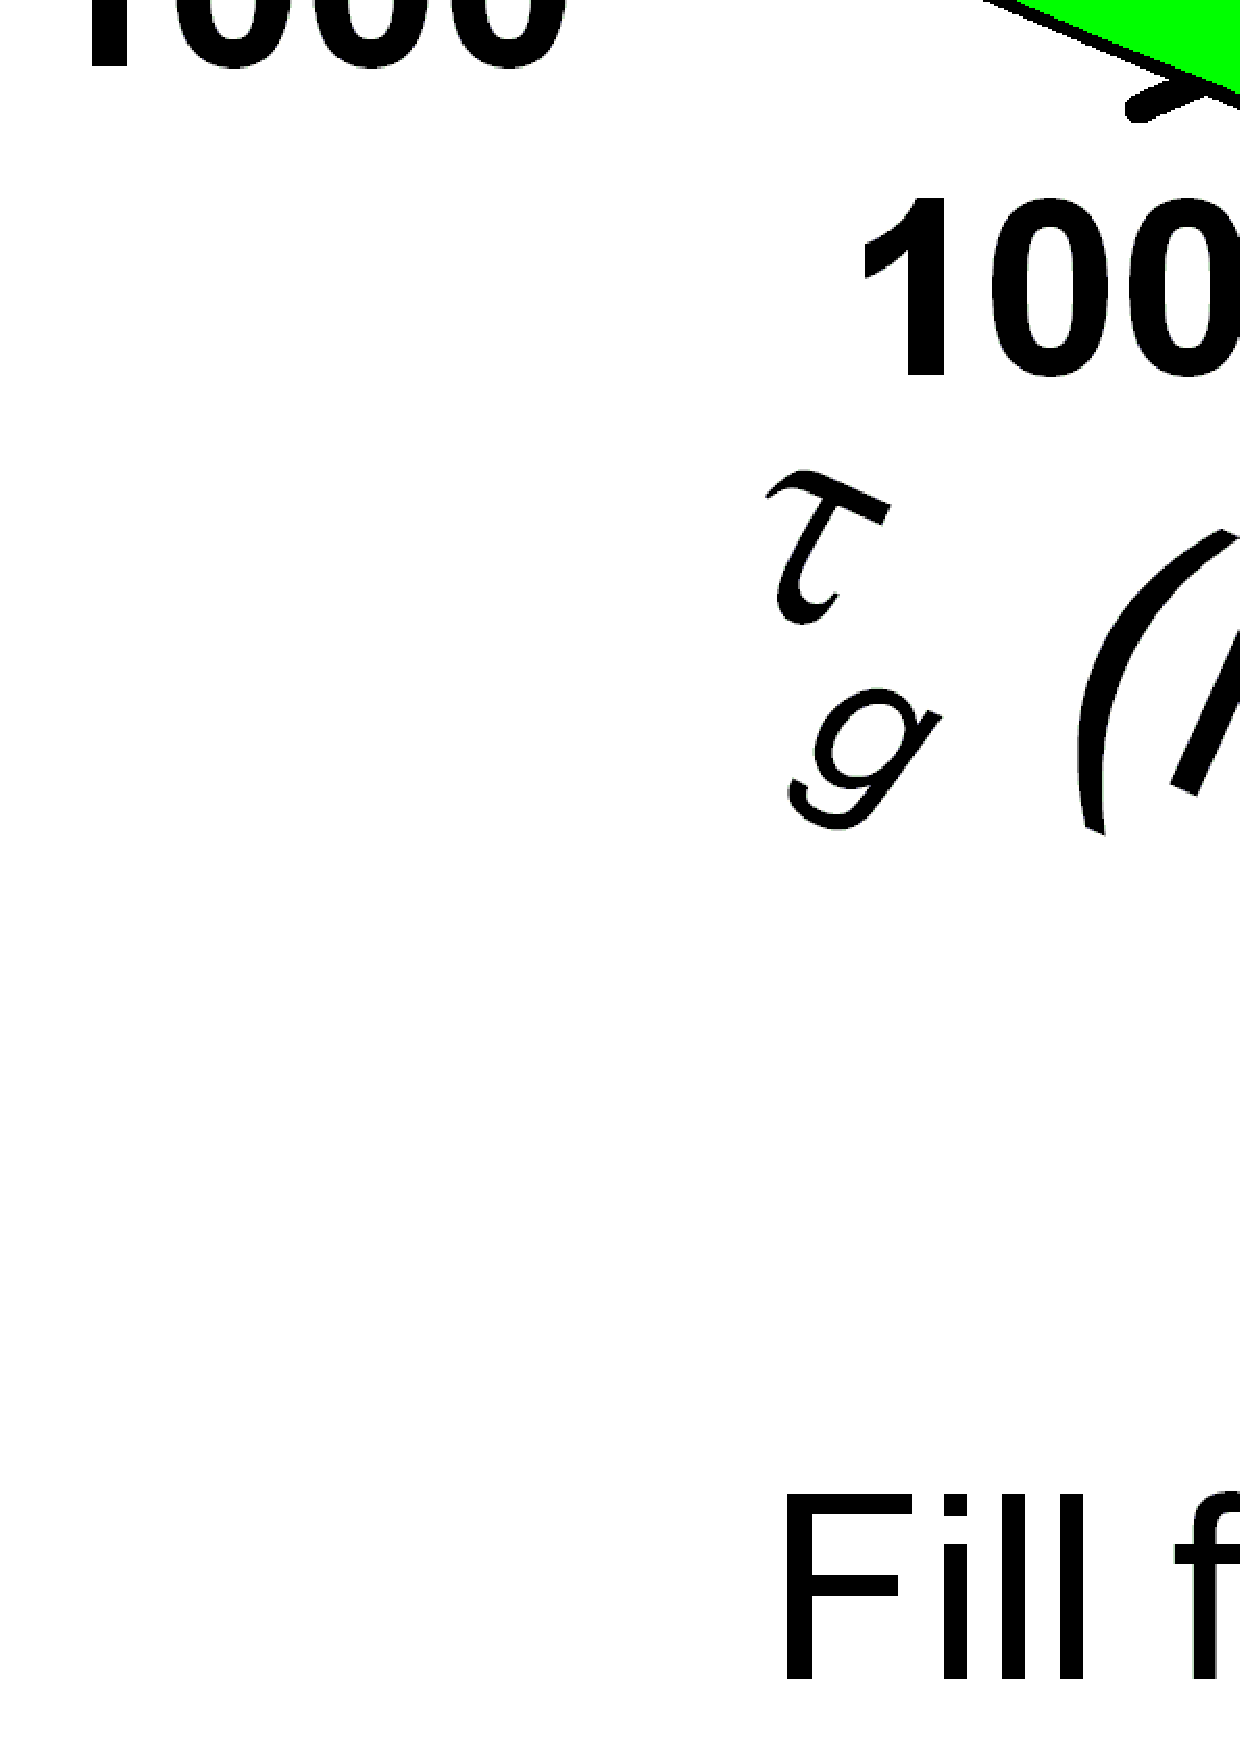
\includegraphics[width=14cm]{olikhFig11}%
\end{center}
\caption{\label{figFF}
Simulated fill factor dependencies on the SCR carrier lifetime and base  carrier lifetime (a), and on the ideality factor and shunt resistance (b).
The constant values $n=2.55$ (a), $R_{sh}=5\times10^3$~$\Omega$ (a), $\tau_n=3\times10^{-6}$~s (b), $\tau_g=5\times10^{-8}$~s (b), and $T=320$~K were used.
}%
\end{figure}

As seen from the Figures~\ref{figVoc}(a) and \ref{figFF}(a),
the $\tau_g$ decrease leads to the decrease in both $V_{oc}$ and $F\!F$.
At the same time, the open--circuit voltage and fill factor dependencies on the base lifetime are weak for the investigated SSCs.
Figs.~\ref{figVoc}(b) and \ref{figFF}(b) show that 
$V_{oc}$ and $FF$ are affected by the both $n_\mathrm{id}$ and $R_{sh}$,
and the effect value considerably depends on shunt resistance value.
For instance, $V_{oc}$ increases with the increase in the ideality factor and both $V_{oc}$ and $FF$ does not almost depend on the shunt resistance value if $R_{sh}>10^5$~$\Omega$ (in the SC15 case).
At the same time,  the open--circuit voltage and fill factor decrease with decrease in the shunt resistance, and only $F\!F$ weakly depends on $n_\mathrm{id}$ if  $R_{sh}\leq10^4$~$\Omega$ (in the SCR4 case).


Therefore the discussed above decrease in $\tau_g$ leads to AI degradation of the both open--circuit voltage and fill factor.
This effect is enhanced by the AI decrease in $R_{sh}$ and partially recovered by the AI increase in $n_\mathrm{id}$ for SC4 and SC15, respectively.

\subsection{Illumination and annealing influence\label{P3}}

Any concrete defect title was not referred as an recombination center in the discussion above.
The additional investigations are necessary to define the type of defects, which are involved in both the recombination and the acousto--defect interaction.

It is known that the most harmful recombination centers in boron--doped Czochralski--grown SSC are the  boron--oxygen related defects \cite{MurphyJAP2011,Kim,LID:BothePP,LIDRev}, iron--boron pairs \cite{MurphyJAP2011,FeB:Vahanissi,FeB:Schmidt} (or another Fe--related trap in the $n^+p$--junctions \cite{TeimurazPSS,TeimurazJAP}), and oxide precipitates \cite{MurphySC2014,Oxide_Schon,MurphyJAP2011,MurphyJAP2012,Oxide:Chen}.
The first two defects are sensitive to an intensive illumination at room temperature.
Thus transformation of boron--oxygen defects by an illumination leads to minority--carrier lifetime degradation (down to as 5 times as small \cite{LIDRev}).
Full lifetime recovery is observed after annealing at 200~$^\circ$C for $10$~min in the dark.
The degradation--recovery cycle can be reiterated \cite{Kim}.
On the other hand, at room temperature, the vast majority of iron exists in iron--boron pairs, which can be readily dissociated under intense illumination to release interstitial iron.
This gives a lifetime change which depends on doping concentration and excess carrier concentration \cite{FeB:Schmidt}.
After the dissociation procedure, the concentration of Fe$_i$ decreases according to \cite{MurphyJAP2011}
\begin{equation}
\label{eqFeB}
N_{Fe}(t)=(N_{Fe,0}-N_{Fe,eq})\exp\left[-1.3\cdot10^{-3}p_p^{\,2/3}\exp\left(-\frac{0.68}{kT}\right)t\right]+N_{Fe,eq}\,,
\end{equation}
where
$N_{Fe,0}$ and $N_{Fe,eq}$ are the concentration after dissociation immediately and equilibrium
concentration which remains a long time after dissociation respectively.



To inspect an availability of boron--oxygen defects and iron--boron pairs the following experimental procedure has been used.
The samples were light soaked under halogen lamp (2 Suns) illumination at approximately 305~K.
The illumination time varied from 1~h to 8~h.
After illumination samples are stored in the dark at room temperature.
To determine the kinetics of SSC parameters the dark $J$--$V$ characteristics have been measured with interval 10--15~min at room temperature over a period 5~h after illumination stopping.
To determine the permanent LID of SSC parameters the dark $J$--$V$ characteristics have been measured in 48~h after illumination.
After accumulated time under illumination had reached 10--15~h the samples were annealed at 200~$^\circ$C for $10$~min in the dark and SSC parameters were determined at room temperature.
After that, the illumination--annealing cycle was repeated.

The results of residual influence of both illumination and annealing on an equilibrium value of SSC parameters are presented on Fig.~\ref{figLight}.
In contrast to other Figures, this contains sample SC--R3 data.
The SC--R3 distinctive features are a low $R_{sh}$ value and a performance of annealing before illumination.
Though the obtained results for SC--R3 are similar to other samples.
One can see that the illumination does not affect a SCR carrier lifetime as well as a base carrier lifetime neither before annealing, nor after.
Illumination induced decrease of ideality factor is commensurable with an accuracy of $n_\mathrm{id}$ determination.
Change of shunt resistance under illumination is most considerable but it reaches $-20$~\% only and does not recur after an  annealing -- see Fig.~\ref{figLight}(d), curve for the sample SC--R4.
Annealing had more efficient influence on SSC parameters and results in  an increment of $\tau_g$ and $R_{sh}$ as well as in a decrement of $\tau_n$ and $n_\mathrm{id}$.
Such behavior of SSC parameters under illumination and annealing action is evident of absence of boron--oxygen defects influence.
The reason of light induced and annealing induced changes  will not be further discussed since this is beyond scope of our study.


\begin{figure}
\begin{center}
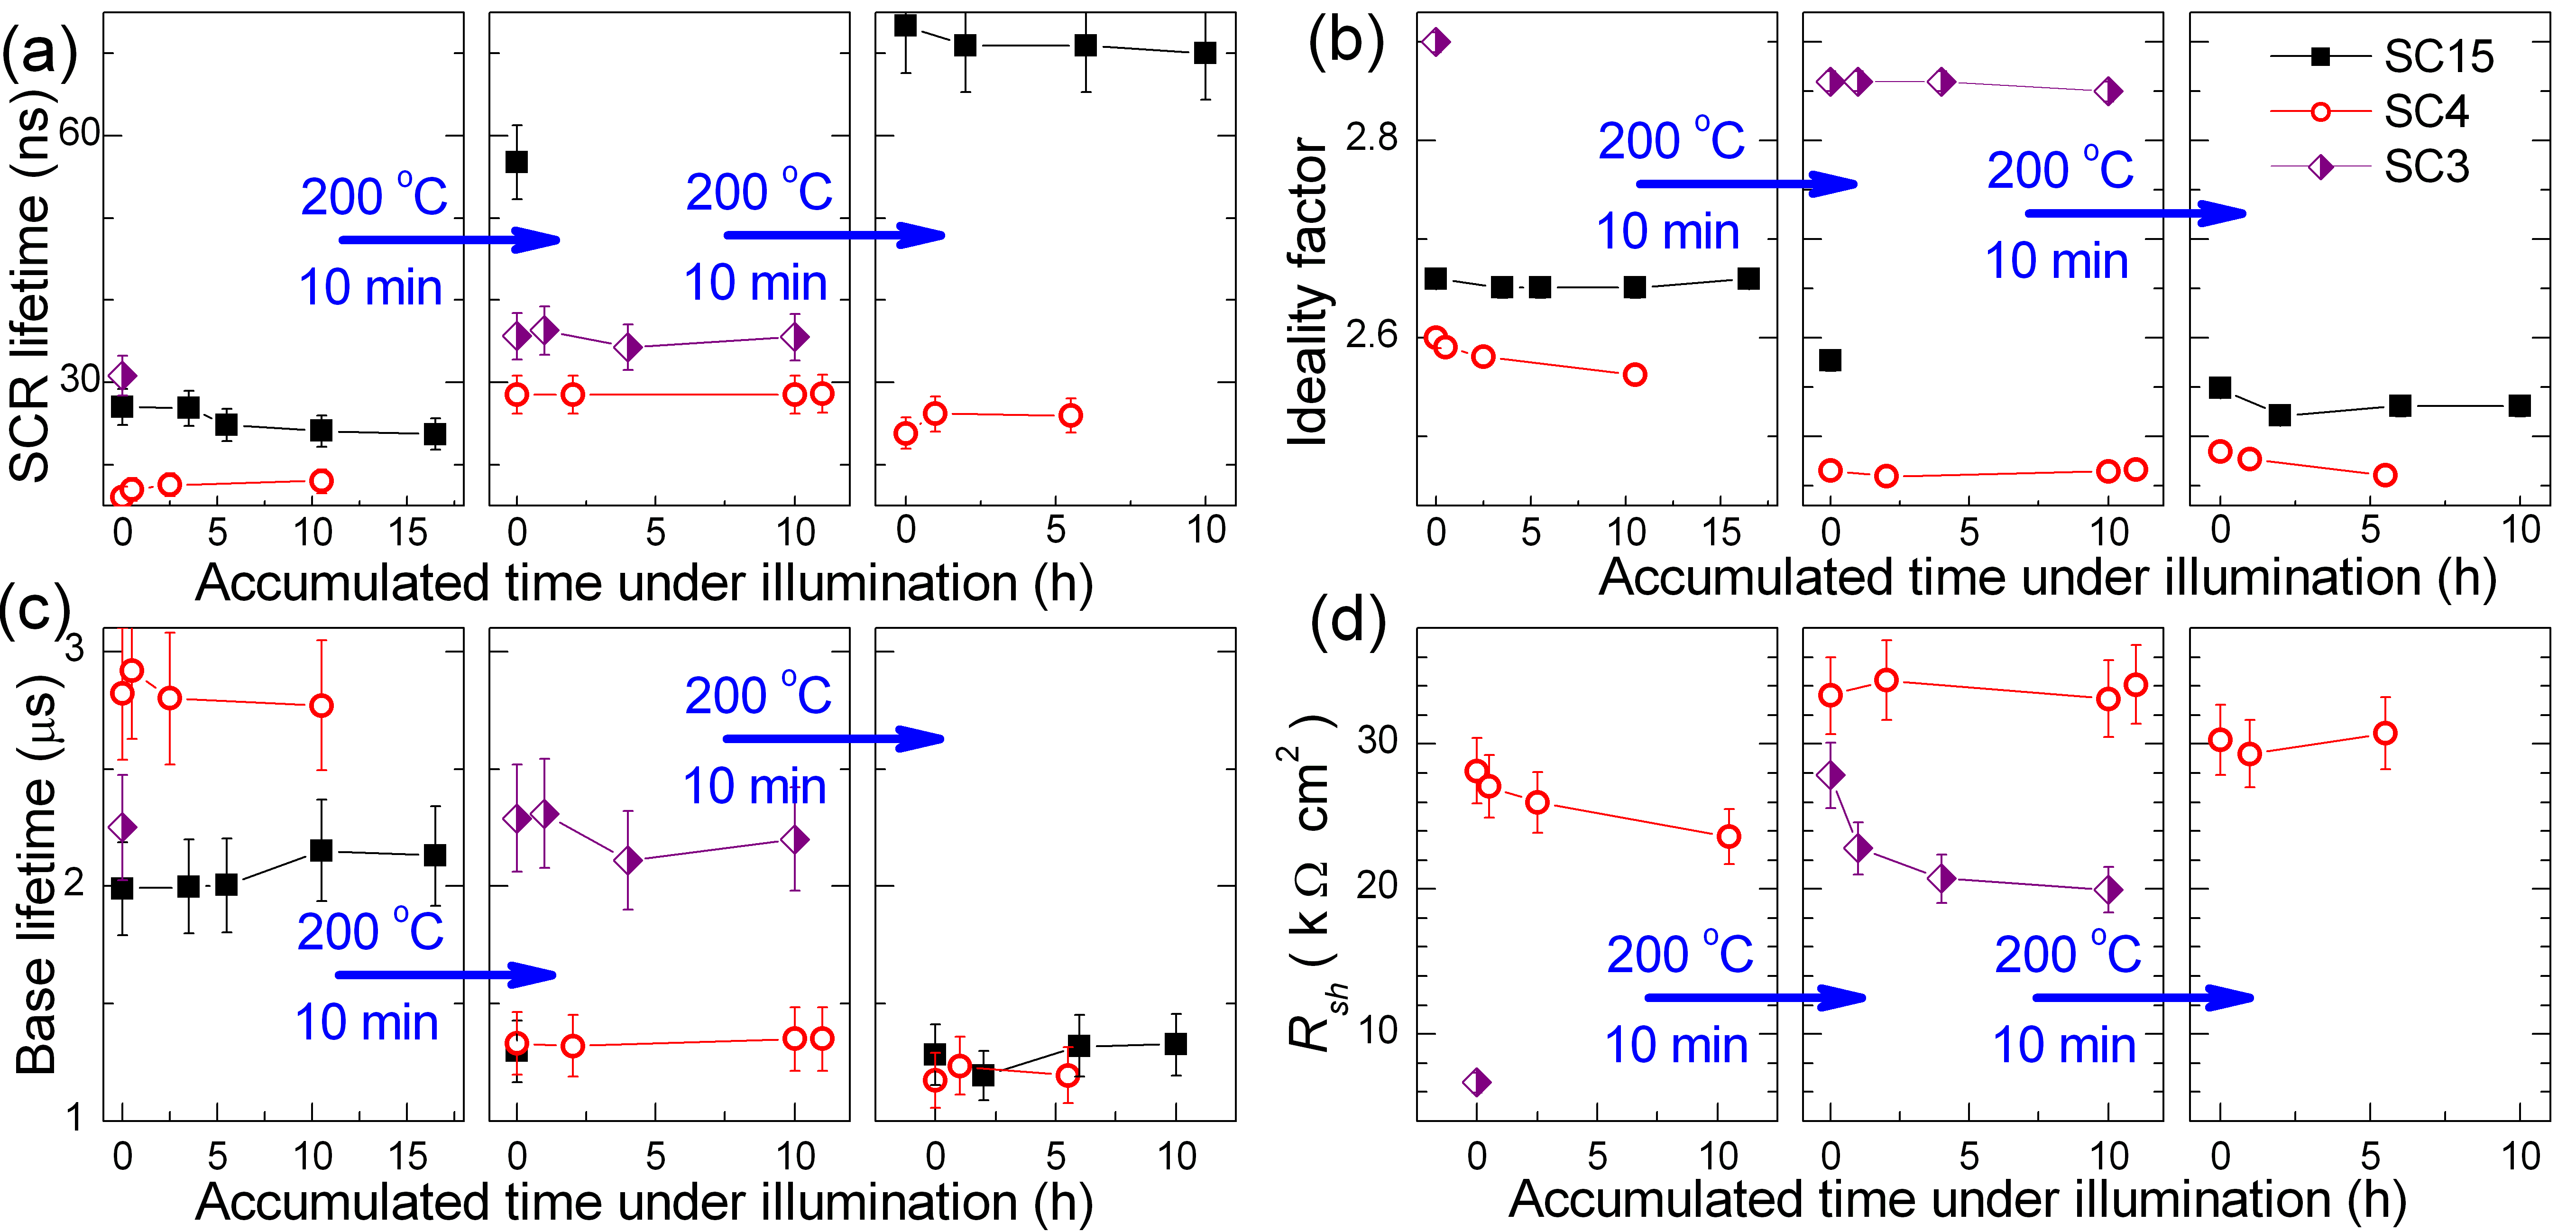
\includegraphics[width=15cm]{olikhFig12}%
\end{center}
\caption{\label{figLight}
Dependencies of SCR carrier lifetime (a), ideality factor (b), base  carrier lifetime (c), and shunt resistance (d) on accumulated illumination time and annealing.
Data were obtained from $J$--$V$ curves which had measured in 48~h after illumination or annealing at $T=295$~K.
Lines only serve as guide to the eye.
}%
\end{figure}

The typical dependencies of SSC parameters versus time since illumination stoping are shown on Fig.~\ref{figAfter}.
As one can see, $\tau_n$ and $R_{sh}$ do not vary practically.
Hence these parameters can not be influenced by iron--boron pairs.
At the same time  $\tau_g$ and $n_\mathrm{id}$ are changing after illumination.
We supposed that the expressions, that have described the both $\tau_g$ and $n_\mathrm{id}$ evolution, were similar to    Eq.~(\ref{eqFeB}) and used the characteristic time $\left[1.3\cdot10^{-3}(1.4\times10^{15})^{\,2/3}\exp\left(-\frac{0.68}{295k}\right)\right]^{-1}=2.53\cdot10^4$~s to plot fitting line on Figs.~\ref{figAfter}(a) and (b).
The fitting is in good agreement with experimental data.
Therefore pairs Fe$_i$B$_s$ can affect a SCR recombination and the acceptor level $E_C-0.23$~eV can be involved in a CDLR recombination process.
Incidentally, pair Fe$_i$B$_s$ is a good candidate for acousto-active defect:
the B is substitutional atom whose volume is smaller than the volume of the matrix atom and $\Delta\Omega_d (\mbox{B}_s)<0$ whereas the interstitial Fe leads to $\Delta\Omega_d (\mbox{Fe}_i)>0$.
On the other hand, the  $\tau_g$ change after illumination is about 10~\% (see Fig.~\ref{figAfter}(a)), whereas a capture cross sections change, which is expected due to pair dissociation, equals to 1.7~times for electrons and 0.04~times for holes \cite{FeB:Schmidt}.
Hence, on our opinion, the pair Fe$_i$B$_s$ is not main reason of a SCR recombination in the investigated samples.


\begin{figure}
\begin{center}
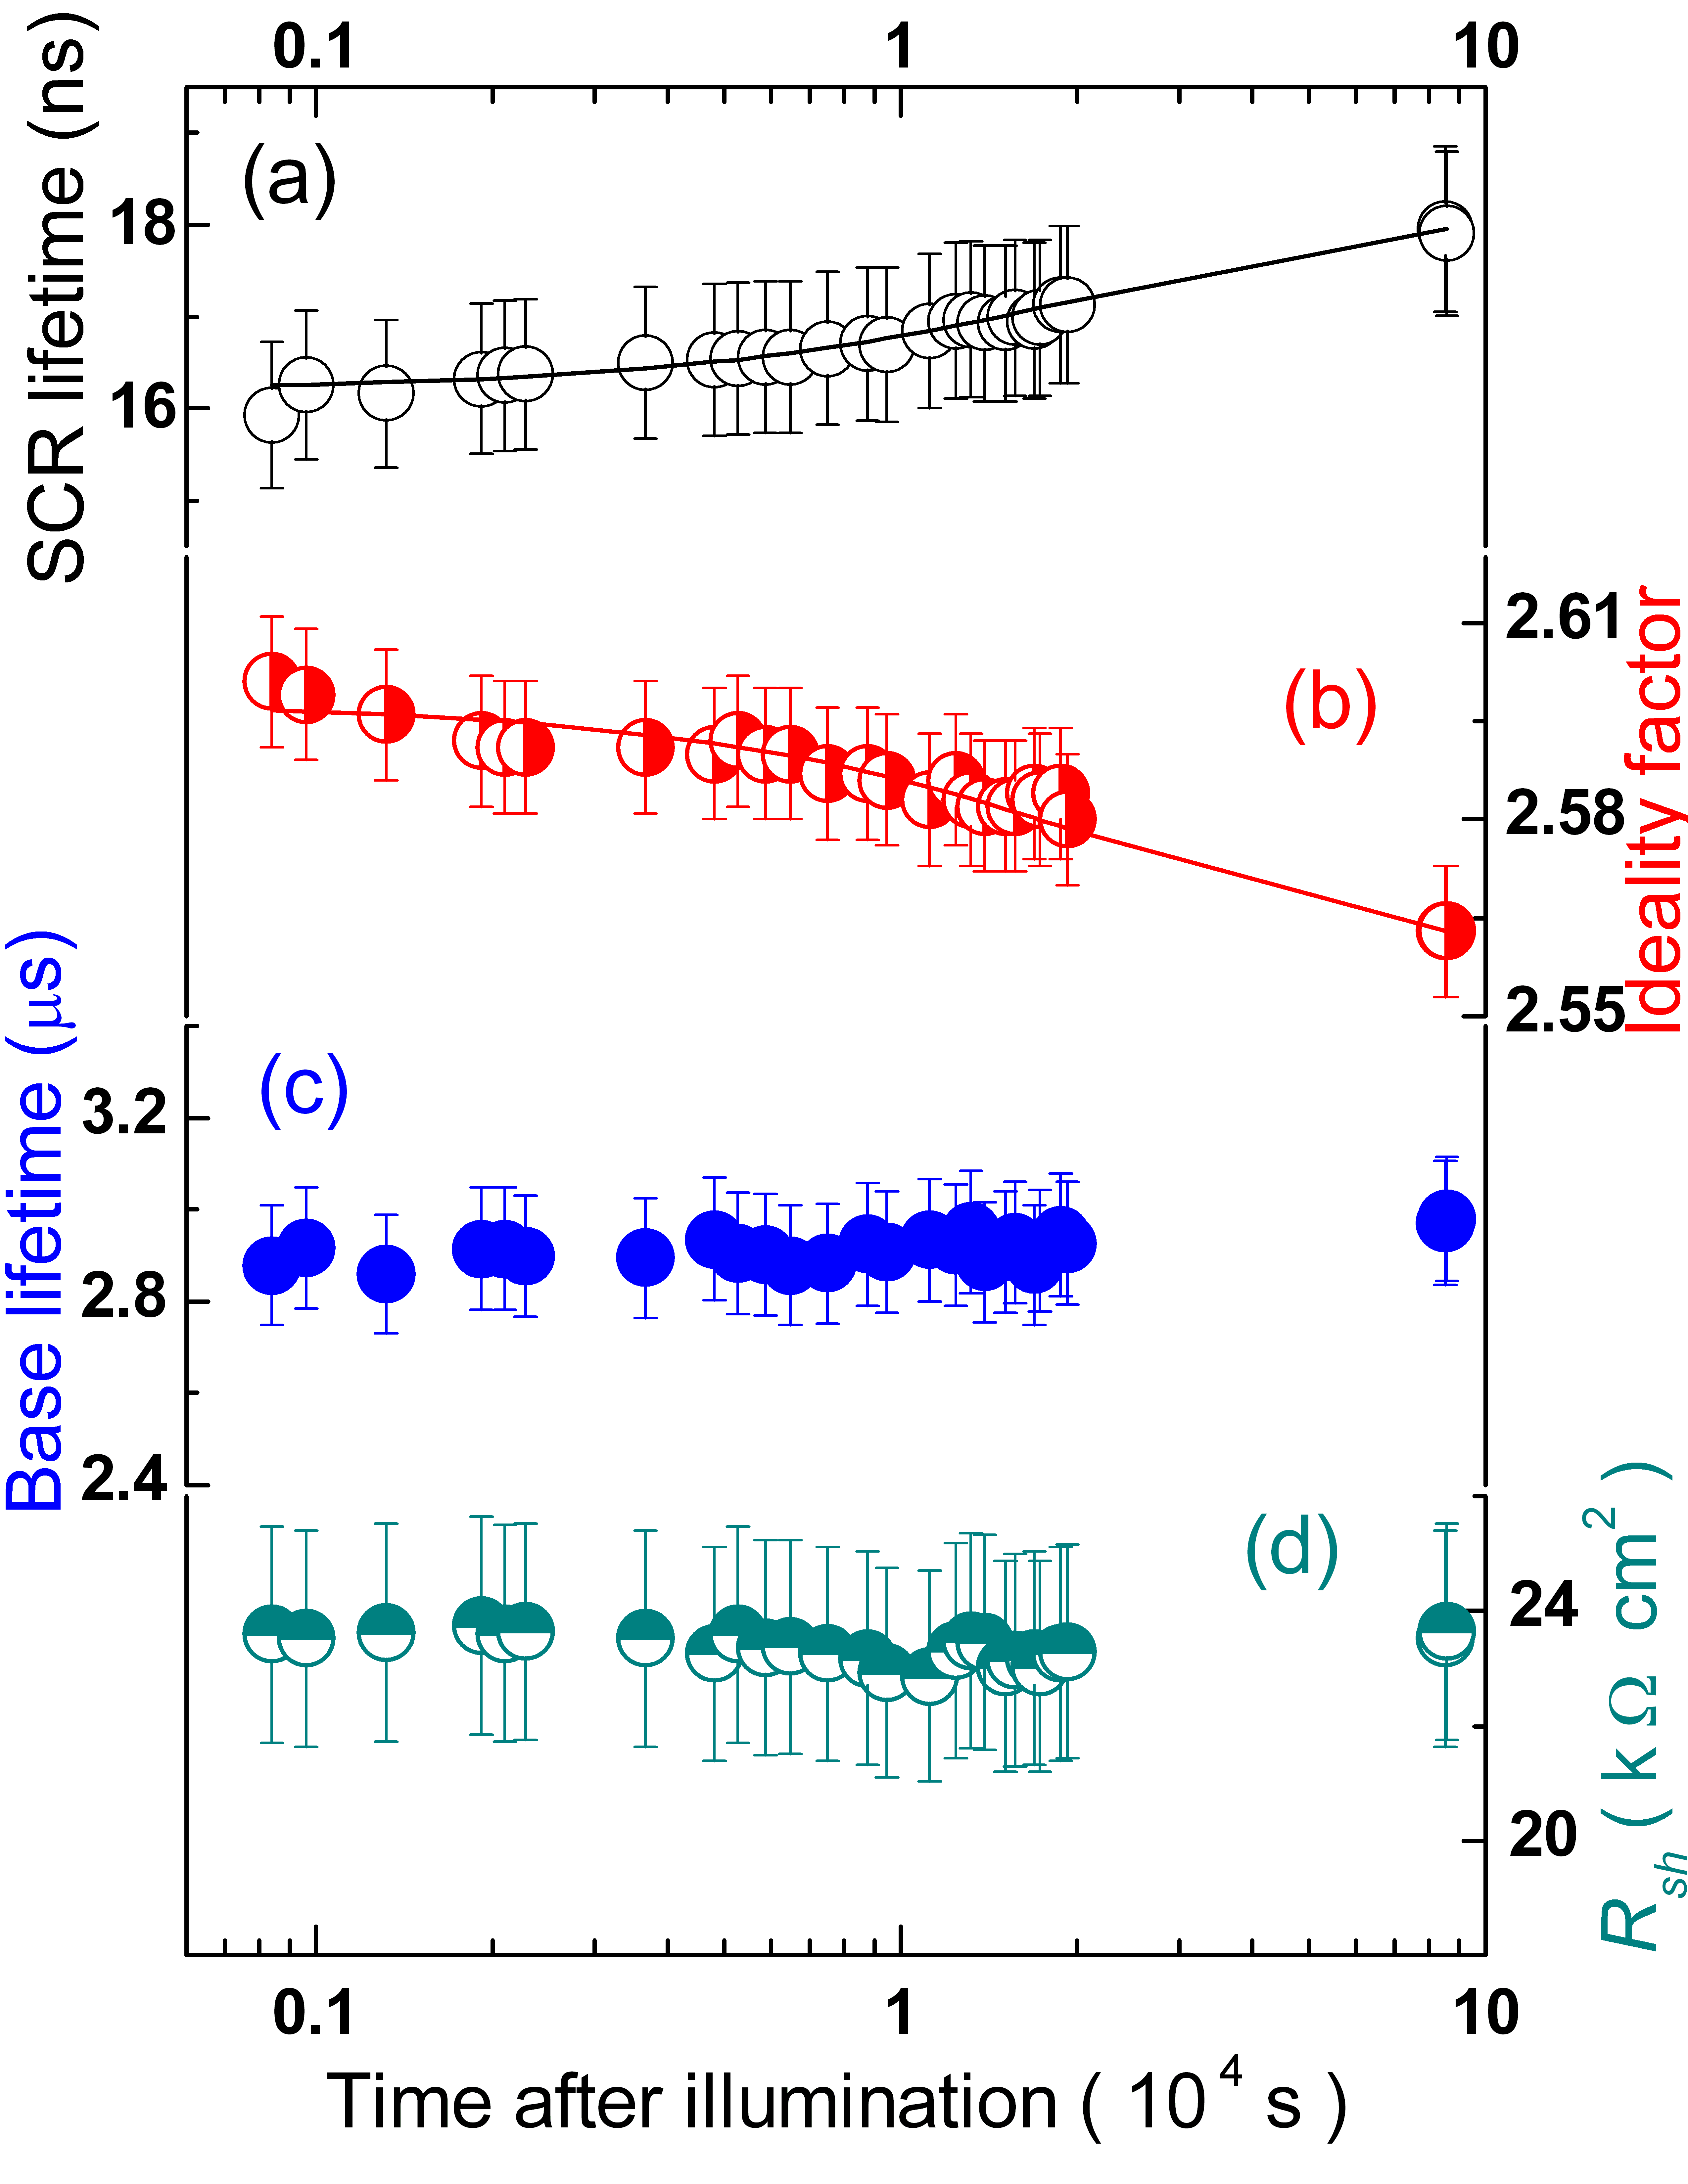
\includegraphics[width=7.5cm]{olikhFig13}%
\end{center}
\caption{\label{figAfter}
SCR carrier lifetime (a), ideality factor (b), base  carrier lifetime (c), and shunt resistance (d) as a function of time since illumination stoping.
Sample SC--R4.
$T=295$~K.
Lines are plotted by using Eq.~(\ref{eqFeB}) and characteristic time $2.53\cdot10^4$~s.
}%
\end{figure}


According to Murphy \emph{et al}.\cite{MurphySC2014,MurphyJAP2012},
the recombination at oxide precipitates cannot be explained by a single two--level defect alone and at least two independent defects are exist.
These defects have single energy levels at $E_V+0.22$~eV and $E_C-0.08$~eV and have $\sigma_n/\sigma_p=157$ and $\sigma_p/\sigma_n=1200$ respectively \cite{MurphyJAP2012}.
So, these defects are suitable for the CDLR recombination process.
Dislocations and stacking faults surround  the oxide precipitates and lead to capture coefficient change as well as to increase the concentrations of two defects, without introducing additional states into the bandgap \cite{MurphySC2014,MurphyJAP2011,MurphyJAP2012} and can provide their acousto--activity.
The oxide precipitates are nonuniformly distributed across a Cz--Si wafer \cite{Oxide_Schon} or a solar cell \cite{Oxide:Chen} and it is the probable reason for a SSC parameters variation from one investigated sample to another.
On the basis of mentioned above, we conclude that the defects, involved in both recombination and acousto--defect interaction are oxide precipitates mainly.





\section{Conclusion}
The experimental investigation of ultrasound influence on the silicon solar cell has been carried out in the temperature range from 290 to 340~K.
The investigation has revealed the acoustically driven reversible degradation of SSC parameters.
It has been found out that the transverse ultrasound waves are more effective tools to affect silicon structure parameters than longitudinal ones.
It has been given evidence that the degradation is due to the recombination amplification under the ultrasound wave action.
The analysis has shown that the acoustically induced increase of carrier capture coefficient of point or extended defects is a reason of observed effects.
The qualitative model of ultrasound influence, which is based on a change of a distance between defects or between components of defect complex under alternating deformation action, is proposed.
It has been shown that the oxide precipitates are most likely defects, which take part in the acousto--defect interaction.
Thus, ultrasound can be an effective tool for controlling silicon structure characteristics.

\section*{References}

\bibliography{olikh}

\end{document}

